% !TeX program = pdflatex
% SCRUM-117: draft integration entrypoint. Compile from repository root.
% Layout adapted from SGU Assignment_report.tex; see docs/report/README.md.
\documentclass[12pt,a4paper]{article}
\usepackage[utf8]{inputenc}
\usepackage[T5]{fontenc}
\usepackage{vntex}
\usepackage[margin=22mm,headheight=30pt]{geometry}
\usepackage{amsmath,amssymb,array,longtable,booktabs,tabularx}
\usepackage{graphicx,pdflscape,fancyhdr,lastpage}
\usepackage[unicode,hidelinks]{hyperref}
\hypersetup{pdftitle={BrewLite Assignment 2 - Draft},pdfauthor={BrewLite team}}
\pagestyle{fancy}
\fancyhf{}
\fancyhead[L]{\small Trường Đại học Sài Gòn -- Khoa Công nghệ Thông tin}
\fancyfoot[L]{\small BrewLite Assignment 2 -- DRAFT}
\fancyfoot[R]{\small Trang \thepage/\pageref{LastPage}}
\setcounter{tocdepth}{2}
\newcommand{\BrewLiteDiagramDir}{docs/diagrams}
\newcommand{\BrewLiteSeqDiagramDir}{docs/report/assets}
\begin{document}
\begin{titlepage}
\begin{center}
TRƯỜNG ĐẠI HỌC SÀI GÒN\\
KHOA CÔNG NGHỆ THÔNG TIN
\vspace{25mm}

{\Large CÔNG NGHỆ PHẦN MỀM\par}
\vspace{12mm}
{\Huge\bfseries BrewLite\par}
\vspace{8mm}
{\Large Assignment 2\par}
{\large Hồ sơ tổng hợp và bàn giao -- bản nháp\par}
\vspace{20mm}

\begin{tabular}{ll}
GVHD, lớp: & Chờ Leader xác nhận\\
Học kỳ: & I -- Năm học 2026--2027 (đề A2 v1.0)\\
Thành viên và MSSV: & Chờ danh sách chính thức\\
Ngày cập nhật hồ sơ: & 11/11/2026\\
Source branch hiện tại: & \texttt{SCRUM-117 / 5021743}\\
Snapshot lịch sử 7dfc7ca; HEAD hiện tại: & \texttt{5021743}\\
Task tài liệu: & SCRUM-117 / A2-T5.4
\end{tabular}
\end{center}
\vfill
\noindent\textbf{DRAFT -- chưa phải báo cáo đã nghiệm thu.}
Đã đối chiếu đề A2 v1.0 và checklist §9.1; production evidence,
release/tag, PDF build và review cuối còn thiếu. Các section kế thừa giữ trạng
thái nguồn, không được hiểu là đã nghiệm thu các task khác.
\end{titlepage}
\tableofcontents
\clearpage
\section*{Nguồn và giới hạn tổng hợp}
\addcontentsline{toc}{section}{Nguồn và giới hạn tổng hợp}
Snapshot lịch sử: \texttt{7dfc7ca996c2eb6190a5ec3e7812f70d441a61cb},
baseline kiểm tra ngày 10/11/2026. Source checkout hiện tại là
\texttt{5021743e99d73c2ce795df72ee5aaa90b04bb0da} (PR \#16), HEAD hiện tại.
branch \texttt{SCRUM-117-production-release-delivery}. Chỉ web Next/proxy/lockfile đổi; các SHA evidence cũ giữ nguyên.
Bố cục A4, bìa, header/footer và mục lục
tái sử dụng cấu trúc template SGU; bỏ dữ liệu minh họa cũ và không tự điền
GVHD/MSSV. Nguồn đề:
\href{https://drive.google.com/file/d/1CYVsexpTXZ6Uyg2FHMRE8lnJHSPkYQmi/view}{Assignment 2 v1.0}
(đọc qua Drive ngày 10/11/2026). Tài liệu Markdown là nguồn vận hành chuẩn:
\href{https://github.com/brewlite-project/brewlite-a2/blob/7dfc7ca996c2eb6190a5ec3e7812f70d441a61cb/docs/architecture/architecture.md}{Architecture tại source snapshot};
các mục SCRUM-117 dùng file \path{docs/deployment.md},
\path{docs/delivery/SCRUM-117-delivery.md} và
\path{docs/delivery/release-notes-A2.md} của branch tài liệu đang review,
chưa có permalink commit. Release source sẽ được cập nhật sau approval.

% SCRUM-99 / A2-T1.1 — fragment; requires vntex, longtable, array, hyperref.
% Canonical content: docs/requirements/context-and-scope.md
\section{Bối cảnh, stakeholder và phạm vi hệ thống BrewLite}
\label{sec:context-and-scope}
\noindent\textbf{Task:} SCRUM-99 / A2-T1.1\par
\noindent\textbf{Trạng thái:} DRAFT -- chờ review; chưa phải biên bản nghiệm thu\par
\noindent\textbf{Ngày soạn:} 08/11/2026\par
\noindent\textbf{Baseline nghiệp vụ:} A1-final -- 1951dc124c83359556f04adb6ba3f0ee9f22fce4\par
\noindent\textbf{Repository đích:} brewlite-project/brewlite-a2; PR base: dev\par

\subsection{Nguồn kế thừa và nguyên tắc sử dụng}

Tài liệu chuẩn hóa bối cảnh, stakeholder, mục tiêu và phạm vi cho Assignment 2 Task 1.1. Nội dung kế thừa Requirements Specification v3.1 và baseline A1-final; không thay thế toàn bộ SRS, không bổ sung nghiệp vụ, API hoặc quyền người dùng.
\par

Requirements v3.1 có business baseline BR-01--BR-06 đã được duyệt, trong khi bản đặc tả ghi trạng thái chờ review. A2 Gap Analysis là bản draft. Việc một yêu cầu nằm trong phạm vi không chứng minh chức năng đó đã triển khai hoặc được nghiệm thu.
\par

Các nguồn dùng trong tài liệu: [S1] Requirements v3.1, mục 3--6, 9.9 và 16; [S2] A2 Gap Analysis, mục 0--1 và 6--7; [S3] README A1 kế thừa trong repo A2, mục 1 và 4; [S4] A2 Implementation Plan. S4 chỉ cung cấp bối cảnh bàn giao, không được dùng để mở rộng baseline nghiệp vụ.
\par

\subsection{Bối cảnh và vấn đề}

BrewLite là ứng dụng web đặt cà phê và đồ uống theo mô hình một cửa hàng (Single-Vendor), phục vụ Guest và Customer. Luồng giá trị chính là xem menu, chọn size/topping, quản lý giỏ hàng, đăng nhập, tạo đơn, thanh toán và xem xác nhận/trạng thái/lịch sử đơn.
\par

Bài toán là duy trì thông tin món, cấu hình, giá và kết quả đơn nhất quán xuyên suốt luồng đặt hàng. Giỏ hàng có thể cũ so với dữ liệu cửa hàng; nhiều khách có thể cùng đặt món cuối; request hoặc thông báo thanh toán có thể được gửi lặp hay đến trễ. Hệ thống cần kiểm tra dữ liệu phía server để tránh tính sai tiền, bán vượt tồn kho và lặp tác động thanh toán hoặc cộng điểm.
\par

Đây là bối cảnh nghiệp vụ của đồ án; chưa có khảo sát định lượng để khẳng định cửa hàng đang gặp một tỷ lệ sai sót cụ thể hoặc BrewLite đã giảm thời gian chờ. A1 cung cấp nền tảng demo local, không phải bằng chứng hệ thống đã vận hành thương mại. [S1 §3--4; S2 §0; S3 §1]
\par

\subsection{Stakeholder, vai trò và nhu cầu}
\begingroup\small
\renewcommand{\arraystretch}{1.2}
\begin{longtable}{>{\raggedright\arraybackslash}p{0.20\linewidth}>{\raggedright\arraybackslash}p{0.43\linewidth}>{\raggedright\arraybackslash}p{0.25\linewidth}}
\hline
\textbf{Stakeholder} & \textbf{Vai trò và nhu cầu} & \textbf{Giới hạn} \\ \hline
\endfirsthead
\textbf{Stakeholder} & \textbf{Vai trò và nhu cầu} & \textbf{Giới hạn} \\ \hline
\endhead
Guest & Người chưa đăng nhập; cần xem menu, giá và tùy chọn size/topping để lựa chọn món. & Phải đăng nhập trước khi tạo Order. \\ \hline
Customer & Người đặt món; cần giỏ hàng, tạo đơn, thanh toán, xác nhận, lịch sử và điểm tích lũy; cần dữ liệu đúng và bảo vệ quyền sở hữu đơn. & Chỉ truy cập tài nguyên thuộc tài khoản; không quyết định giá, tồn kho hay kết quả thanh toán. \\ \hline
Quản lý cửa hàng / PO mô phỏng & Stakeholder xác định giá trị, ưu tiên backlog và chấp nhận increment; cần phạm vi rõ và quy tắc nhất quán. & Không suy ra có tài khoản hay UI quản trị; không gán PO cho thành viên khi chưa được xác nhận. \\ \hline
Nhân viên quầy / Barista & Stakeholder liên quan đến chuẩn bị và hoàn tất đồ uống; cần hiểu các trạng thái PREPARING, READY, COMPLETED. & UI Barista nằm ngoài MVP; stakeholder nghiệp vụ không đồng nghĩa actor có giao diện đã triển khai. \\ \hline
VNPay Sandbox & Hệ thống ngoài tham gia redirect và trao đổi kết quả IPN/QueryDR; cần dữ liệu giao dịch và thông báo được xác minh theo hợp đồng tích hợp. & Chỉ Sandbox; không giao dịch tiền thật. Mock và ZERO\_AMOUNT là cơ chế nội bộ, không phải actor ngoài. \\ \hline
Nhóm phát triển & Phân tích, thiết kế, triển khai, review và kiểm thử; cần nguồn yêu cầu thống nhất, khả năng truy vết và tái tạo môi trường. & Lịch sử A1 không thay thế bằng chứng review và kiểm chứng A2. \\ \hline
Giảng viên & Đánh giá đồ án; cần tạo phẩm, demo và bằng chứng có thể kiểm tra theo tiêu chí Assignment. & Không mặc định đã nghiệm thu khi mới có tài liệu hoặc test lịch sử. \\ \hline
\end{longtable}
\endgroup

Guest và Customer là actor sử dụng web chính; VNPay Sandbox là actor hệ thống ngoài. Các stakeholder còn lại có lợi ích và trách nhiệm liên quan nhưng không mặc nhiên có quyền thao tác trong ứng dụng. [S1 §5--6; S2 §0]
\par

\subsection{Mục tiêu sản phẩm}
\begingroup\small
\renewcommand{\arraystretch}{1.2}
\begin{longtable}{>{\raggedright\arraybackslash}p{0.24\linewidth}>{\raggedright\arraybackslash}p{0.68\linewidth}}
\hline
\textbf{Mục tiêu} & \textbf{Kết quả mong muốn trong baseline} \\ \hline
\endfirsthead
\textbf{Mục tiêu} & \textbf{Kết quả mong muốn trong baseline} \\ \hline
\endhead
G1 -- Đặt món rõ ràng & Khách xem món/giá, chọn size/topping và quản lý giỏ trước khi tạo đơn. \\ \hline
G2 -- Đơn hàng nhất quán & Server kiểm tra giỏ, tính lại giá, lưu thông tin đơn và kiểm soát tồn kho để tránh oversell. \\ \hline
G3 -- Thanh toán có kiểm soát & Kết quả thanh toán được xác minh; request lặp không lặp tác động; retry và trường hợp chưa rõ kết quả tuân thủ baseline. \\ \hline
G4 -- Theo dõi và bảo vệ dữ liệu & Customer xem kết quả/lịch sử đơn của mình; JWT và ownership bảo vệ nghiệp vụ cần đăng nhập; coupon/điểm tuân thủ quy tắc đã có. \\ \hline
G5 -- Có thể đánh giá và bàn giao & Tài liệu mô tả đúng hệ thống, môi trường có thể tái tạo và bằng chứng được ghi theo trạng thái thực tế. \\ \hline
\end{longtable}
\endgroup

Đây là mục tiêu và kết quả mong muốn, không phải tuyên bố các tiêu chí đã PASS. Ngưỡng đo, FR/NFR chi tiết và Acceptance Criteria sẽ được chuẩn hóa trong SRS của task tương ứng, không tự phát minh tại Task 1.1. [S1 §1, §3--6; S2 §1]
\par

\subsection{Ranh giới hệ thống}

Bên trong BrewLite: Web Client Next.js, Backend API NestJS, dữ liệu PostgreSQL qua Prisma và các cơ chế nội bộ phục vụ Order, Inventory, Payment, Promotion/Loyalty. Docker Compose là cách tái tạo môi trường kế thừa A1.
\par

Web Client hiển thị và gửi yêu cầu; Backend là nơi quyết định giá, kiểm tra tồn kho, quyền truy cập và thay đổi trạng thái nghiệp vụ. Không tin giá, userId hay kết quả thanh toán do client tự khai.
\par

Bên ngoài BrewLite: Guest/Customer và VNPay Sandbox. VNPay Sandbox là provider mặc định. Mock CARD/WALLET chỉ phục vụ automated test/demo khi backend cho phép trong môi trường không phải production và luôn bị tắt ở production. ZERO\_AMOUNT xử lý nội bộ đơn 0 VND, độc lập với Mock. Không tự fallback sang Mock khi VNPay PENDING hoặc chưa rõ kết quả. [S1 §3, §9.9, §16]
\par

\subsection{In Scope -- phạm vi nghiệp vụ kế thừa}
\begingroup\small
\renewcommand{\arraystretch}{1.2}
\begin{longtable}{>{\raggedright\arraybackslash}p{0.20\linewidth}>{\raggedright\arraybackslash}p{0.43\linewidth}>{\raggedright\arraybackslash}p{0.25\linewidth}}
\hline
\textbf{Nhóm} & \textbf{Nội dung được mô tả trong phạm vi} & \textbf{Nguồn} \\ \hline
\endfirsthead
\textbf{Nhóm} & \textbf{Nội dung được mô tả trong phạm vi} & \textbf{Nguồn} \\ \hline
\endhead
Identity & Đăng ký/đăng nhập JWT, băm mật khẩu Argon2id và bảo vệ API/quyền sở hữu dữ liệu. & S1 §4.1, §7.1 \\ \hline
Catalog và Cart & Menu, chi tiết, size/topping; thêm/sửa/xóa giỏ và tổng tạm; server tính lại khi tạo đơn. & S1 §4.1, §6 F02--F03 \\ \hline
Order và Inventory & Tạo đơn, kiểm tra hợp lệ, snapshot, trạng thái/lịch sử, chống oversell và hết hạn/hoàn tài nguyên theo lifecycle. & S1 §6 F04--F05 \\ \hline
Payment & VNPay Sandbox; xác minh IPN/QueryDR; PENDING/SUCCESS/FAILED; idempotency, retry có kiểm soát, grace và reconciliation; bảo lưu Mock test/demo và ZERO\_AMOUNT. & S1 §4.1, §9.9, §16 \\ \hline
Promotion và Loyalty & Kiểm tra coupon, giới hạn lượt dùng, tính giảm giá và cộng điểm sau thanh toán hợp lệ, không cộng trùng. & S1 §6 F07 \\ \hline
Kiểm chứng và bàn giao kế thừa & Kiểm thử, Docker Compose, README và demo; phân biệt bằng chứng lịch sử A1 với kiểm chứng A2. & S1 §4.1; S2 §0 \\ \hline
\end{longtable}
\endgroup

Bảng xác định phạm vi yêu cầu, không xác nhận mức hoàn thành. Phạm vi QueryDR được bảo lưu nhưng Sandbox E2E còn Deferred; các giới hạn ở mục 9 áp dụng cho mọi phát biểu về tính năng.
\par

\subsection{Out of Scope và Deferred}
\begingroup\small
\renewcommand{\arraystretch}{1.2}
\begin{longtable}{>{\raggedright\arraybackslash}p{0.24\linewidth}>{\raggedright\arraybackslash}p{0.68\linewidth}}
\hline
\textbf{Nội dung} & \textbf{Ranh giới áp dụng} \\ \hline
\endfirsthead
\textbf{Nội dung} & \textbf{Ranh giới áp dụng} \\ \hline
\endhead
Thanh toán tiền thật và refund tự động & Không kích hoạt cổng thanh toán production hoặc giao dịch thật; không tự thêm nghiệp vụ refund. \\ \hline
Multi-vendor, microservices, mobile native & Giữ mô hình một cửa hàng và stack hiện có. \\ \hline
Seller/Admin phức tạp và UI Barista & Module Seller/Admin phức tạp và UI Barista nằm ngoài phạm vi sản phẩm baseline; vòng đời trạng thái đơn vẫn được mô tả theo yêu cầu kế thừa. \\ \hline
Vận chuyển và định vị thời gian thực & Không bổ sung Last-Mile, tracking hoặc nghiệp vụ giao nhận. \\ \hline
ERP/POS và quản lý nguyên liệu đầy đủ & Tồn kho chỉ phục vụ phạm vi chống oversell và lifecycle tài nguyên của baseline. \\ \hline
Forgot/Reset Password; hủy đơn chủ động & Forgot/Reset Password và FR-ORD-005 tiếp tục Deferred; không mô tả endpoint/UI tương ứng như đã có. \\ \hline
\end{longtable}
\endgroup

A1 từng defer deployment chính thức và CI/CD nâng cao; không được suy diễn rằng các mục này nằm ngoài toàn bộ Assignment 2. Task 1.1 chỉ ghi nhận sự phân biệt giữa phạm vi sản phẩm kế thừa và yêu cầu bàn giao A2. Advanced monitoring không được tự bổ sung như tính năng đã có. [S1 §4.2, §6 F04; S2 §3--5; S4]
\par

\subsection{Giả định và ràng buộc}

Giả định phân tích: A1-final là baseline nghiệp vụ dùng để kế thừa; chưa có quyết định được duyệt cho thay đổi nghiệp vụ ngoài baseline trong Task 1.1. Mọi đề xuất thay đổi cần được ghi riêng và review trước khi cập nhật phạm vi.
\par

Giữ Next.js, NestJS, TypeScript, PostgreSQL, Prisma và Docker; không thực hiện refactor hay đổi cấu trúc frontend/backend trong task tài liệu này.
\par

Guest có thể xem menu; tạo đơn, thanh toán và xem lịch sử cần JWT hợp lệ và kiểm tra quyền sở hữu. Backend là nguồn quyết định giá và trạng thái.
\par

Môi trường A2 cần tách khỏi A1 về Compose project và DB/volume; không kế thừa việc container A1 đang chạy thành bằng chứng A2. Hosting và chính sách payment demo A2 còn cần quyết định theo planning.
\par

Tài liệu phải phân biệt yêu cầu, hiện trạng được ghi nhận và bằng chứng nghiệm thu. Không đánh dấu PASS, Done hoặc Approved nếu chưa có review và chứng cứ tương ứng. [S1 §3--5; S2 §0, §7; S4]
\par

\subsection{Rủi ro và giới hạn kiểm chứng}
\begingroup\small
\renewcommand{\arraystretch}{1.2}
\begin{longtable}{>{\raggedright\arraybackslash}p{0.24\linewidth}>{\raggedright\arraybackslash}p{0.68\linewidth}}
\hline
\textbf{Rủi ro / giới hạn} & \textbf{Cách thể hiện và xử lý trong Task 1.1} \\ \hline
\endfirsthead
\textbf{Rủi ro / giới hạn} & \textbf{Cách thể hiện và xử lý trong Task 1.1} \\ \hline
\endhead
Scope creep từ stakeholder cửa hàng & Ghi vai trò và nhu cầu nhưng không biến thành tính năng Admin/Barista mới. \\ \hline
Nhầm yêu cầu với chức năng hoàn thành & Dùng ngôn ngữ mục tiêu/yêu cầu; không dùng “đã hoàn tất” nếu thiếu bằng chứng. \\ \hline
QueryDR Sandbox E2E còn Deferred & Bảo lưu phạm vi đối soát; không dùng synthetic/local tests để tuyên bố đã chạy Sandbox E2E. \\ \hline
Sai lệch payment-status API được Gap Analysis ghi nhận & Giữ trạng thái cần đối chiếu ở A2; không khẳng định đã có route hoặc đã sửa; xử lý ở task kỹ thuật riêng. \\ \hline
A1 local demo; production/CI/CD/PWA A2 chưa được xác nhận & Không ghi đã deploy, đã có pipeline hoặc đạt PWA; yêu cầu kiểm chứng tại task A2 tương ứng. \\ \hline
Nguồn tài liệu chưa chốt nghiệm thu & Ghi v3.1 chờ review đặc tả, business baseline đã duyệt; Gap Analysis draft; PR/reviewer/merge là chứng cứ còn cần bổ sung. \\ \hline
\end{longtable}
\endgroup

Các giới hạn trên kế thừa S2, không phải kết quả chạy lại toàn bộ hệ thống trong SCRUM-99. Task này không sửa lỗi kỹ thuật hoặc thay đổi business rule để khép các gap. [S2 §0, §5--7]
\par

\subsection{Tạo phẩm và điều kiện review Task 1.1}

Tạo phẩm chuẩn: docs/requirements/context-and-scope.md. Phần báo cáo tương ứng: docs/report/sections/context-and-scope.tex; đây là fragment dùng trong mẫu SGU, không phải báo cáo A2 hoàn chỉnh.
\par

Công việc thuộc các task A2 khác: SRS chi tiết, UC, diagram, kiến trúc, CI/CD và deployment được thực hiện trong các task tương ứng, không triển khai trong SCRUM-99. Đây là giới hạn công việc của Task 1.1, không phải danh sách loại trừ của sản phẩm A2. Production/CI/CD là yêu cầu bàn giao A2 theo planning, chưa được ghi nhận là đã nghiệm thu. [S2; S4]
\par

Review cần kiểm tra bối cảnh/mục tiêu rõ; từng stakeholder có vai trò và nhu cầu; In Scope/Out of Scope nhất quán với A1-final; không mô tả chức năng chưa kiểm chứng như đã hoàn thành; nội dung Markdown và LaTeX thống nhất.
\par

Thay đổi cần được đưa lên nhánh riêng từ dev có mã SCRUM-99, tạo PR về dev và có review theo quy trình nhóm. Tài liệu này chưa xác nhận đã commit, push, mở PR, review hay merge; không tự đánh dấu Jira Done.
\par

\subsection{Tài liệu tham chiếu}

Phiên bản nguồn [S1]--[S4] được cố định tại commit 8b4224a907091529ca954c8b0792406cb8a0d9f2 của repository brewlite-project/brewlite-a2, đọc ngày 08/11/2026. Đây là commit nguồn tài liệu A2; baseline nghiệp vụ A1-final vẫn là 1951dc124c83359556f04adb6ba3f0ee9f22fce4.
\par

[S1] BrewLite Requirements Specification v3.1, cập nhật 30/10/2026. Nguồn tham chiếu chính: docs/BrewLite\_Requirements\_Specification\_v3.1.docx. Bản trong docs/docs\_Phase2/ có cùng nội dung tại commit nguồn được chốt bên dưới.
\par

[S2] docs/planning/A2\_Gap\_Analysis.md -- DRAFT, 08/11/2026.
\par

[S3] README.md -- tài liệu A1 kế thừa, không phải chứng nhận production A2.
\par

[S4] docs/planning/A2\_Implementation\_Plan.md -- PROPOSED / NOT APPROVED, 08/11/2026.
\par

\begin{itemize}
\item \href{https://github.com/brewlite-project/brewlite-a2/blob/8b4224a907091529ca954c8b0792406cb8a0d9f2/docs/BrewLite_Requirements_Specification_v3.1.docx}{Requirements v3.1}
\item \href{https://github.com/brewlite-project/brewlite-a2/blob/8b4224a907091529ca954c8b0792406cb8a0d9f2/docs/planning/A2_Gap_Analysis.md}{A2 Gap Analysis}
\item \href{https://github.com/brewlite-project/brewlite-a2/blob/8b4224a907091529ca954c8b0792406cb8a0d9f2/README.md}{README}
\item \href{https://github.com/brewlite-project/brewlite-a2/blob/8b4224a907091529ca954c8b0792406cb8a0d9f2/docs/planning/A2_Implementation_Plan.md}{A2 Implementation Plan}
\end{itemize}

\clearpage
% SCRUM-102 / A2-T1.2 -- fragment; requires vntex, longtable, array, hyperref.
% Canonical catalog and complete traceability: docs/requirements/srs.md
\section{Yêu cầu chức năng và phi chức năng}
\label{sec:requirements-summary}
\noindent\textbf{Task:} SCRUM-102 / A2-T1.2\par
\noindent\textbf{Trạng thái:} DRAFT -- chờ review và xác nhận các gap; chưa phải biên bản nghiệm thu\par
\noindent\textbf{Ngày soạn:} 08/11/2026\par
\noindent\textbf{Baseline nghiệp vụ:} A1-final -- 1951dc124c83359556f04adb6ba3f0ee9f22fce4\par
\noindent\textbf{Danh mục đầy đủ:} \texttt{docs/requirements/srs.md}\par

\subsection{Cách chuẩn hóa và ưu tiên}

Requirements Specification v3.1 có 46 ID FR và 49 ID NFR. Danh mục A2 giữ nguyên ID nguồn; tách FR-CAT-001 thành baseline danh sách và pagination, và FR-PRO-001 thành kiểm tra coupon khi tạo Order và coupon preview. Vì vậy danh mục có 48 dòng FR và 49 dòng NFR, không làm mất yêu cầu nguồn. Mapping UC dựa trên nội dung: UC-PRO-001 xem điểm/ưu đãi; UC-PRO-002 xem trước coupon. Bảng AC, US/UC và vị trí kiểm chứng đầy đủ nằm trong SRS.
\par

MUST/SHOULD được lấy từ mức ưu tiên và quy tắc trong nguồn. Với NFR không có mức ưu tiên tường minh, dấu MUST* là phân loại dự thảo dựa trên ràng buộc bảo mật, toàn vẹn, tin cậy hoặc khả năng tái tạo; cần reviewer xác nhận. Không tự tạo nhóm Could hoặc Won't. MVP theo 10 task A1 và phần mở rộng Phase 2 đều kế thừa In Scope; state machine, idempotency, concurrency/inventory và coupon/loyalty thuộc Task 10. “Chưa triển khai” hoặc “chưa có bằng chứng” không đổi mức ưu tiên.
\par

\subsection{Một số yêu cầu tiêu biểu}
\begingroup\small
\renewcommand{\arraystretch}{1.2}
\begin{longtable}{>{\raggedright\arraybackslash}p{0.10\linewidth}>{\raggedright\arraybackslash}p{0.30\linewidth}>{\raggedright\arraybackslash}p{0.16\linewidth}>{\raggedright\arraybackslash}p{0.34\linewidth}}
\hline
\textbf{ID} & \textbf{Yêu cầu} & \textbf{Ưu tiên / phạm vi} & \textbf{Tiêu chí và đối chiếu} \\ \hline
\endfirsthead
\textbf{ID} & \textbf{Yêu cầu} & \textbf{Ưu tiên / phạm vi} & \textbf{Tiêu chí và đối chiếu} \\ \hline
\endhead
FR-01 & Guest đăng ký Customer với email chuẩn hóa, email duy nhất và password được hash Argon2id. & MUST; MVP & Dữ liệu hợp lệ tạo đúng một Customer; email trùng không tạo bản ghi thứ hai. V-AUTH; SRS AC-A2-001. \\ \hline
FR-21 & Order chỉ chuyển theo state machine; transition và side effects được xử lý nguyên tử. & MUST; Task 10 & Transition ngoài ma trận bị từ chối; trạng thái terminal không bị ghi đè. V-ORDER/V-PAY; SRS AC-A2-021. \\ \hline
FR-27 & Các Order đồng thời không được oversell; thiếu stock phải rollback toàn transaction. & MUST; Task 10 & PostgreSQL concurrency test chứng minh không có stock âm hay Order/resource một phần. V-INV; SRS AC-A2-027. \\ \hline
FR-32 & Idempotency-Key ràng buộc theo user; replay cùng payload không lặp payment attempt hoặc side effect. & MUST; Task 10 & Kiểm thử replay và key đồng thời trên PostgreSQL; payload khác tuân contract. V-PAY; SRS AC-A2-032. \\ \hline
FR-34 & UI phân biệt pending/unknown, success, failure cuối và kết quả hết hạn; không tin Return URL. & MUST; Phase 2 & API v4 yêu cầu GET payment status nhưng PaymentsController ở A1-final chưa có route tương ứng; đây là gap implementation. V-STATUS; SRS AC-A2-034. \\ \hline
FR-38 & QueryDR dùng chung finalization; kết quả không rõ không được suy thành FAILED. & MUST; Phase 2 & Automated/synthetic cases kiểm tra state và side effects; QueryDR Sandbox E2E và lost-IPN recovery đang Deferred theo ADR. V-VNP; SRS AC-A2-038. \\ \hline
FR-23 & Hủy chủ động bởi Customer được ghi nhận riêng, không đồng nhất với tự hết hạn Order. & SHOULD; Deferred & Auto-expiration và release tài nguyên vẫn thuộc In Scope; không mặc định có Cancel API/UI. V-ORDER; SRS AC-A2-023. \\ \hline
FR-43 & Coupon preview là yêu cầu riêng với coupon validation lúc tạo Order. & SHOULD; Deferred theo S1/S3/S6 & SCRUM-96 xác nhận implementation decisions cùng request/response/error contract; route/test files có trong A1 nhưng không chứng minh acceptance. Leader cần chốt scope/acceptance A2. V-PROMO; SRS AC-A2-043. \\ \hline
FR-45 & Loyalty points chỉ cộng đúng một lần khi thanh toán hợp lệ làm Order chuyển PAID. & MUST; Phase 2 & Điều kiện theo provider: VNPay trong grace cần payDate đúng hạn và Order chưa CANCELLED; late/ineligible không hồi sinh/cộng điểm; ZERO_AMOUNT eligible kết thúc với 0 điểm, không gateway/grace; replay không cộng lặp. SRS AC-A2-045. \\ \hline
NFR-01 & JWT được xác minh và ownership được thực thi phía server. & MUST*; bảo mật & Thử hai Customer truy cập chéo bằng integration test; dữ liệu của chủ khác không lộ. V-AUTH/V-ORDER/V-PAY; SRS AC-A2-049. \\ \hline
NFR-03 & Password dùng Argon2id; DB được phép lưu hash/salt, nhưng không persist plaintext hoặc trả/log plaintext/hash. & MUST*; bảo mật & Đối chiếu DB, API response và log capture khi đăng ký/đăng nhập. SRS AC-A2-051. \\ \hline
NFR-10 & Tạo Order, finalization, release, coupon và loyalty phải atomic. & MUST*; nhất quán & Inject lỗi ở từng bước trên PostgreSQL; xác nhận rollback, không có side effect một phần. V-ORDER/V-INV/V-PAY/V-PROMO; SRS AC-A2-058. \\ \hline
NFR-21 & Mục tiêu xử lý nội bộ dưới 500 ms áp dụng trên dữ liệu mẫu/Mock. & MUST; hiệu năng & Đo xử lý server-side trong môi trường/dữ liệu mẫu được ghi rõ; không áp SLA tổng thể cho redirect/IPN/QueryDR bất đồng bộ. V-PAY/V-ORDER; SRS AC-A2-069. \\ \hline
NFR-40 & Môi trường cần tái tạo từ clone sạch theo hướng dẫn Compose và seed. & MUST*; vận hành & Chạy trên DB/volume riêng, ghi cấu hình, health và seed evidence; không khẳng định đã đạt trước khi chạy. V-OPS; SRS AC-A2-088. \\ \hline
\end{longtable}
\endgroup

\subsection{Giới hạn nguồn và các gap cần xác nhận}

Các tài liệu chưa có cùng trạng thái approval: Requirements v3.1 ghi chờ review nhưng BR-01--BR-06 được duyệt; US/AC Phase 2 v2.3 ghi Review Fixed; Use Case Phase 2 v3.1 là Candidate; API Contract v4.0 có header NOT APPROVED trong khi phần mở đầu nói API Design Baseline Approved. Tài liệu này giữ nguyên trạng thái từng nguồn và để Leader xác nhận chính xác phạm vi approval; không tuyên bố mọi tài liệu hoặc implementation đã được Approved.
\par

Payment Status là requirement của API v4.0 và frontend có gọi route, nhưng controller A1-final chưa có GET /payments/:paymentId/status. QueryDR vẫn In Scope/MUST; nghiệm thu Sandbox E2E cùng phục hồi mất IPN được ADR chuyển sang A2, nên test giả lập không được dùng làm bằng chứng Sandbox PASS. Hủy chủ động tiếp tục Deferred; tự hết hạn và hoàn tài nguyên vẫn thuộc phạm vi. Với coupon preview, S1/S3/S6 giữ SHOULD/Deferred; SCRUM-96 xác nhận implementation decisions cùng request/response/error contract riêng cho endpoint, nhưng không đổi priority hoặc approval tổng thể API. A1 có route/test files, song đây không phải bằng chứng feature đã được nghiệm thu; Leader cần xác nhận product scope và acceptance status A2.
\par

NFR-PERF-001 đặt mục tiêu dưới 500 ms cho xử lý nội bộ trên dữ liệu mẫu/Mock. Không suy rộng thành thời gian thanh toán VNPay bất đồng bộ, p95, uptime hoặc cam kết tải. Mỗi NFR quan trọng cần môi trường đo và bằng chứng tương ứng như nêu trong SRS.
\par

\noindent\textbf{Nguồn được ghim:} [S1] Requirements v3.1; [S3] User Stories/AC Phase 2 v2.3; [S5] Use Case Phase 2 v3.1 PDF; [S6] API Contract v3.0; [S7] API Contract v4.0; [S9] addenda và quyết định liên quan. Tất cả dùng snapshot A1-final commit 1951dc124c83359556f04adb6ba3f0ee9f22fce4; trạng thái và liên kết chi tiết nằm trong SRS. [\href{https://github.com/brewlite-project/brewlite-a2/blob/1951dc124c83359556f04adb6ba3f0ee9f22fce4/docs/BrewLite_Requirements_Specification_v3.1.docx}{S1}] [\href{https://github.com/brewlite-project/brewlite-a2/blob/1951dc124c83359556f04adb6ba3f0ee9f22fce4/docs/docs_Phase2/BrewLite_User_Stories_Acceptance_Criteria_Phase2.docx}{S3}] [\href{https://github.com/brewlite-project/brewlite-a2/blob/1951dc124c83359556f04adb6ba3f0ee9f22fce4/docs/docs_Phase2/BrewLite_Use_Case_Specification_v3.1_VNPay_Phase_2\%20.pdf}{S5}] [\href{https://github.com/brewlite-project/brewlite-a2/blob/1951dc124c83359556f04adb6ba3f0ee9f22fce4/docs/api/BrewLite_API_Contract_v3.0.md}{S6}] [\href{https://github.com/brewlite-project/brewlite-a2/blob/1951dc124c83359556f04adb6ba3f0ee9f22fce4/docs/api/BrewLite_API_Contract_v4.0.md}{S7}] [\href{https://github.com/brewlite-project/brewlite-a2/blob/1951dc124c83359556f04adb6ba3f0ee9f22fce4/docs/decisions/ADR-P2-QueryDR-Sandbox-E2E-Deferred.md}{ADR QueryDR}]\par

\noindent Tài liệu đang ở trạng thái DRAFT. Chưa chạy build/test ứng dụng vì thay đổi chỉ gồm tài liệu. Fragment này chưa biên dịch; kiểm chứng bố cục sẽ thực hiện khi tích hợp báo cáo tổng hợp SGU.
\par

\clearpage
% BrewLite A2 — Task 1.3. Fragment for inclusion into the A2 report.
% Requires in main preamble: \usepackage[utf8]{inputenc} (pdfLaTeX, if needed),
% \usepackage{longtable}, \usepackage{array}; Vietnamese UTF-8 engine/package per report template.
\section{Đặc tả Use Case trọng tâm --- Checkout}
\label{sec:a2-checkout}

\subsection{Mục tiêu và phạm vi}
Use Case \texttt{UC-A2-CHECKOUT-001} (mã đề xuất) mô tả quy trình Customer
xác nhận giỏ, tạo Order và thanh toán đến khi nhận được kết quả đáng tin cậy,
hoặc đến trạng thái chờ đối soát/hết hạn. Phạm vi kế thừa UC-ORD-001 và
UC-PAY-001 của BrewLite A1, nhưng sử dụng các quy tắc Phase~2 từ Requirements
v3.1 và API Contract v4.0. Tài liệu này không thay đổi API hay schema.

\subsection{Actor, Trigger và điều kiện}
\begin{description}
\item[Primary actor:] Customer đã đăng nhập.
\item[External supporting actor:] VNPay Sandbox (chỉ nhánh VNPay).
\item[Supporting components:] Frontend, Auth, Order, Pricing, Inventory, Coupon,
Payment, Finalization, Expiration/Reconciliation và Database.
\item[Trigger:] Customer nhấn Đặt hàng từ giỏ, sau đó chọn thanh toán.
\item[Precondition:] Customer có JWT hợp lệ để tạo Order và gửi được giỏ;
điều kiện tồn kho, coupon, Order active và expiry được xác minh trong flow.
\item[Success postcondition:] Order PAID, tối đa một Payment SUCCESS,
coupon CONSUMED/loyalty một lần và không trừ stock lần hai.
\item[Alternate postcondition:] Terminal FAILED trong TTL giữ tồn/coupon;
unknown giữ Payment PENDING; Order CANCELLED khi đủ điều kiện expiry thì
release tài nguyên đúng một lần.
\end{description}

\subsection{Main Success Flow}
\begin{enumerate}
\item Customer xác thực và gửi giỏ cùng coupon (nếu có) đến Order API.
\item Backend xác minh giỏ, Order active, giá/size/topping, tồn kho và coupon.
\item Backend tính tiền theo catalog, tạo Order PENDING cùng snapshot,
trừ/giữ tài nguyên nguyên tử; đặt expiresAt bằng createdAt cộng 15 phút.
\item Với totalVnd dương, Customer chọn VNPay; backend kiểm ownership,
TTL, idempotency và attempt trạng thái hiện tại rồi khởi tạo VNPay PENDING.
\item VNPay nhận thanh toán, gửi IPN; backend xác minh chữ ký, merchant,
TxnRef, amount, outcome và paid time. Return URL không đủ xác nhận SUCCESS.
\item Shared Finalization xác minh SUCCESS đúng hạn, Order chưa CANCELLED;
Payment SUCCESS, Order PAID, coupon CONSUMED, loyalty đúng một lần.
\item Frontend đọc Payment Status/Order History từ backend và hiển thị
kết quả; chỉ xóa giỏ khi đã xác nhận PAID.
\end{enumerate}

\subsection{Alternative và Exception Flows}
\begin{itemize}
\item Zero amount: dùng ZERO\_AMOUNT nội bộ, không gọi VNPay, pointsEarned=0.
\item Mock: chỉ khi được bật trong non-production và không có VNPay PENDING.
\item Verified FAILED: Order PAYMENT\_FAILED khi còn hạn; retry chỉ với attempt
mới sau xác nhận terminal failed.
\item TTL/Grace: không initiation từ expiresAt; VNPay PENDING có grace 5 phút
để đối soát thanh toán đã phát sinh đúng hạn. Hết grace còn unknown thì
Order CANCELLED/release, Payment có thể vẫn PENDING.
\item Wrong JWT/ownership: 401/404; invalid cart/stock/coupon: validation/409;
active Order: 409 PENDING\_ORDER\_EXISTS; idempotency mismatch: 409.
\item Invalid IPN, timeout, QueryDR unknown: không tự PAID/FAILED;
late financial SUCCESS sau CANCELLED lưu evidence, không hồi sinh Order.
\end{itemize}

\subsection{Traceability và giới hạn xác minh}
Chi tiết mọi nhánh, mã lỗi và traceability nằm trong tệp
\texttt{docs/requirements/A2\_T1.3\_Checkout\_Use\_Case\_Specification.md}.
Chưa đối chiếu được A2 Task 1.2 và source \texttt{brewlite-a2/dev}; các route
trong API Contract v4.0 là căn cứ thiết kế, không mặc định đã triển khai.

\clearpage
% SCRUM-103 / A2-T2.1 — Fragment cho báo cáo Assignment 2.
% Canonical content: docs/diagrams/A2_T2.1_Activity_Diagram_Checkout.md
% Source diagrams:
%   - docs/diagrams/activity-checkout.puml (Tổng thể End-to-End)
%   - docs/diagrams/activity-checkout-phase1-order.puml (Pha 1: Tạo Order & Khởi tạo thanh toán)
%   - docs/diagrams/activity-checkout-phase2-payment.puml (Pha 2A: Tương tác VNPay, Return URL độc lập & Kết quả Customer)
%   - docs/diagrams/activity-checkout-phase3-reconciliation.puml (Pha 2B: Xử lý IPN, Chu kỳ Scheduler Đối soát & TTL/Grace)
% Rendered exports:
%   - docs/diagrams/activity-checkout*.svg / .pdf
%   - docs/report/assets/activity-checkout*.pdf
% Yêu cầu gói trong preamble chính: \usepackage{graphicx}, \usepackage{longtable}, \usepackage{array}

\section{Activity Diagram --- Luồng Checkout (\texttt{UC-A2-CHECKOUT-001})}
\label{sec:a2-activity-checkout}

\noindent\textbf{Task:} SCRUM-103 / A2-T2.1\par
\noindent\textbf{Trạng thái:} DRAFT -- đã cập nhật phản hồi Review lần 2 của PR \#4 (\texttt{R-01}..\texttt{R-06} \& tối ưu bố cục trình bày)\par
\noindent\textbf{Ngày soạn:} 08/11/2026\par
\noindent\textbf{Baseline đối chiếu:} \texttt{A1-final} (\texttt{1951dc124c83359556f04adb6ba3f0ee9f22fce4})\par
\noindent\textbf{Tệp nguồn \& kết xuất:} \texttt{docs/diagrams/activity-checkout.puml}, \texttt{docs/diagrams/activity-checkout-phase1-order.puml}, \texttt{docs/diagrams/activity-checkout-phase2-payment.puml}, \texttt{docs/diagrams/activity-checkout-phase3-reconciliation.puml} (cùng các bản xuất \texttt{.svg} và \texttt{.pdf} đồng bộ)\par

\subsection{Mục tiêu và nguyên tắc kế thừa từ Assignment 1}

Sơ đồ hoạt động (Activity Diagram) của Task~2.1 mô hình hóa luồng nghiệp vụ end-to-end cho Use Case trọng tâm \texttt{UC-A2-CHECKOUT-001} (\emph{Đặt hàng và thanh toán}), kế thừa bốn sơ đồ con trong bộ tạo phẩm Assignment~1 (\texttt{docs/diagram/Activity-Final.drawio.svg}: \texttt{AD-02} Quy trình đặt món tổng quan, \texttt{AD-03} Tạo đơn hàng, \texttt{AD-04} Thanh toán và \texttt{AD-06} Hủy đơn hàng quá 15 phút) và chuẩn hóa theo Requirements Specification v3.1 cùng API Contract v4.0.
\par

So với phiên bản A1 vốn chỉ chia hai phân vùng tổng quát (\emph{Người dùng} và \emph{Hệ thống}) và chỉ mô tả thanh toán giả lập (\texttt{CARD}/\texttt{WALLET}), sơ đồ chuẩn hóa ở Assignment~2 giải quyết trọn vẹn các yêu cầu của mục Task~2.1:
\begin{itemize}
  \item Tách rõ \textbf{5 swimlane} theo đúng kiến trúc thực tế: \texttt{Customer}, \texttt{Next.js Frontend}, \texttt{NestJS Backend}, \texttt{PostgreSQL DB} và actor ngoài \texttt{VNPay Sandbox}.
  \item Chuẩn hóa toàn bộ các \textbf{Decision Node (D1--D22)} theo quy tắc thống nhất (\texttt{R-02}): nhánh \texttt{then} luôn mang nhãn khẳng định \texttt{Có (...)} khớp trực tiếp với câu hỏi nghi vấn trong hình thoi, và nhánh \texttt{else} luôn mang nhãn phủ định \texttt{Không (...)}.
  \item Biểu diễn \textbf{Luồng 1 (Browser Redirect qua Return URL)} và \textbf{Luồng 2 (Server-to-Server IPN / Scheduler đối soát nội bộ)} là hai luồng hoàn toàn độc lập (\texttt{R-03}), sử dụng \texttt{fork ... end merge} và kết thúc độc lập ở luồng nền (\texttt{stop}), loại bỏ điểm đồng bộ giả (Join Bar) để phản ánh đúng thực tế Backend vẫn hoàn tất đơn ngay cả khi \texttt{Customer} đóng trình duyệt.
  \item Mô hình hóa rõ \textbf{vòng lặp chu kỳ Scheduler đánh giá lại theo thời gian (\texttt{R-04})}: khi giao dịch còn \texttt{PENDING} trước mốc \(E = \text{createdAt} + 15\text{m}\) hoặc vừa bước vào cửa sổ Grace \(5\text{ phút}\) \([E, G)\) với \(G = E + 5\text{m}\) (\texttt{RECONCILING}), hệ thống lưu trạng thái vào Database và đi qua bước chờ sự kiện tiếp theo (IPN đến muộn hoặc chu kỳ kích hoạt kế tiếp của \texttt{PaymentReconciliationScheduler} / \texttt{OrderExpirationService}) trước khi đánh giá lại các mốc \(E\) và \(G\).
  \item Đảm bảo tất cả các nhánh thanh toán --- bao gồm \textbf{VNPay Sandbox (\texttt{Main Flow})}, \textbf{đơn hàng \(0\,\text{đ}\) (\texttt{AF-03: ZERO\_AMOUNT})} và \textbf{chế độ Mock test/demo (\texttt{AF-04})} --- đều đi qua bước lưu bền vững tại \texttt{PostgreSQL DB}, đồng bộ về \texttt{Next.js Frontend} để hiển thị giao diện và kết thúc tại \texttt{Customer} (\texttt{R-05}).
  \item Chia sơ đồ thành \textbf{3 hình tách pha rõ nét} (\texttt{Pha 1}, \texttt{Pha 2A}, \texttt{Pha 2B}) bên cạnh bản tổng thể end-to-end để tối ưu tỉ lệ hiển thị trên trang báo cáo A4 (\texttt{R-06}).
\end{itemize}

\subsection{Phân vùng trách nhiệm (Swimlanes) và các nút quyết định chính}

\begingroup\small
\renewcommand{\arraystretch}{1.2}
\begin{longtable}{>{\raggedright\arraybackslash}p{0.20\linewidth}>{\raggedright\arraybackslash}p{0.44\linewidth}>{\raggedright\arraybackslash}p{0.28\linewidth}}
\hline
\textbf{Swimlane} & \textbf{Hành động chính trên sơ đồ} & \textbf{Ràng buộc / Bất biến} \\ \hline
\endfirsthead
\hline
\textbf{Swimlane} & \textbf{Hành động chính trên sơ đồ} & \textbf{Ràng buộc / Bất biến} \\ \hline
\endhead
\texttt{Customer} & Mở giỏ hàng, nhập mã coupon (tùy chọn), nhấn Đặt hàng; xác nhận thanh toán hoặc chọn Retry; thao tác trên cổng VNPay Sandbox; nhận kết quả cuối cùng cho cả 3 nhánh (\texttt{VNPay}, \texttt{ZERO\_AMOUNT}, \texttt{Mock}). & Chỉ được Retry khi \texttt{Order == PAYMENT\_FAILED}, còn hạn \(\text{now} < E\) và không có cờ đối soát/ngoại lệ tài chính. \\ \hline
\texttt{Next.js Frontend} & Kiểm tra JWT client-side; gửi \texttt{POST /orders}; giữ giỏ hàng cho đến khi \texttt{Order == PAID}; sinh \texttt{Idempotency-Key} (8..64 ký tự); redirect sang VNPay; nhận Return URL độc lập và gọi \texttt{GET /orders/me} (bounded polling); hiển thị kết quả cuối cùng cho \texttt{Customer}. & Không tự coi Return URL là \texttt{PAID} (\texttt{EF-11}); không tự xóa giỏ khi giao dịch còn \texttt{PENDING}. \\ \hline
\texttt{NestJS Backend} & Thực thi \texttt{JwtAuthGuard}, \texttt{ValidationPipe}, \texttt{MockPaymentGuard}; tính giá authoritative (\texttt{round-half-up}); kiểm tra 1 Order active, \texttt{Idempotency-Key} và TTL; khởi tạo VNPay; xử lý độc lập ở nền qua IPN (\texttt{GET /payments/vnpay/ipn}) hoặc chu kỳ Scheduler đối soát nội bộ; thực thi \texttt{Shared Finalization}. & Không tin cậy giá/discount từ client; khóa bản ghi theo thứ tự chuẩn để chống race condition (\texttt{EF-13 / BR-C05}). \\ \hline
\texttt{PostgreSQL DB} & Kiểm tra Order active, tồn kho và coupon trong transaction; lưu snapshot \texttt{Order}/\texttt{OrderItem}; trừ/hoàn stock; chuyển trạng thái coupon (\texttt{HELD} \(\rightarrow\) \texttt{CONSUMED} hoặc release); cập nhật \texttt{Payment} và điểm tích lũy nguyên tử. & Rollback toàn bộ khi lỗi (\texttt{EF-15}); mỗi tài nguyên chỉ được trừ/tiêu thụ hoặc hoàn trả đúng một lần. \\ \hline
\texttt{VNPay Sandbox} & Hiển thị cổng thanh toán cho nhánh \texttt{totalVnd > 0}; kích hoạt 2 luồng độc lập: (1) Browser Redirect qua Return URL về Frontend và (2) Server-to-Server IPN về Backend. & Chỉ tham gia trên nhánh VNPay; không tham gia nhánh \texttt{ZERO\_AMOUNT} hoặc Mock. \\ \hline
\end{longtable}
\endgroup

\subsection{Tóm tắt luồng hoạt động theo 3 sơ đồ tách pha}

\begin{enumerate}
  \item \textbf{Pha 1 --- Tạo Order \texttt{PENDING}, giữ tài nguyên và khởi tạo thanh toán (Hình~\ref{fig:a2-activity-checkout-phase1}):}
  \begin{itemize}
    \item \emph{Kiểm tra đăng nhập và tạo đơn (\texttt{POST /orders}):} \texttt{Next.js Frontend} kiểm tra phiên JWT (\textbf{D1}: \texttt{Đã đăng nhập?} \(\rightarrow\) \texttt{Có} gửi \texttt{POST /orders} / \texttt{Không [EF-01]} yêu cầu đăng nhập, giữ giỏ). Tại \texttt{NestJS Backend}, \textbf{D2} (\texttt{JWT \& DTO hợp lệ?}) trả \texttt{401/400} nếu \texttt{Không}. Trong DB Transaction nguyên tử, hệ thống xét \textbf{D3} (\texttt{Đã có Order active?} \(\rightarrow\) nếu \texttt{Có} trả \texttt{409 PENDING\_ORDER\_EXISTS} --- \texttt{EF-05 / BR-C02}) và \textbf{D4} (\texttt{Đủ stock \& Coupon hợp lệ?} \(\rightarrow\) nếu \texttt{Không} thì rollback nguyên tử và trả \texttt{409 INSUFFICIENT\_STOCK} hoặc \texttt{400/409} lỗi coupon --- \texttt{EF-04 / EF-15}). Nếu \texttt{Có}, hệ thống tính giá authoritative phía server (\texttt{BR-C01}), đặt \(\text{expiresAt} = E = \text{createdAt} + 15\text{m}\), tạo \texttt{Order (PENDING)}, trừ tồn kho và giữ coupon (\texttt{HELD}).
    \item \emph{Phân nhánh khởi tạo thanh toán:} Sau khi kiểm tra quyền sở hữu (\texttt{EF-02}), \texttt{Idempotency-Key} (\texttt{AF-10 / EF-06}), hạn TTL (\texttt{EF-08}) và cờ chặn (\texttt{EF-07}) tại \textbf{D5} (\texttt{Đủ điều kiện thanh toán?}), luồng rẽ qua:
    \begin{itemize}
      \item \textbf{D6 (\texttt{Đơn hàng 0đ (totalVnd == 0)?}):} Nếu \texttt{Có [AF-03, BR-C07]}, xử lý \texttt{POST /payments/zero-amount}, commit nguyên tử \texttt{Payment = SUCCESS (0đ)}, \texttt{Order = PAID}, \texttt{Coupon HELD \(\rightarrow\) CONSUMED}, \texttt{loyaltyPointsEarned = 0} rồi chuyển sang Pha~2A để hiển thị cho \texttt{Customer}.
      \item \textbf{D7--D9 (\texttt{Dùng chế độ Mock [AF-04]?}):} Nếu \texttt{Có}, xét \textbf{D8} (\texttt{Cho phép chạy Mock?}: nếu \texttt{Không [BR-C09]} trả \texttt{403 MOCK\_PAYMENT\_DISABLED}). Tại \textbf{D9} (\texttt{Thẻ 0002 / Ví 0000 từ chối?}), nếu \texttt{Có} thì commit \texttt{Payment = FAILED}, \texttt{Order = PAYMENT\_FAILED}; nếu \texttt{Không} thì commit \texttt{Payment = SUCCESS}, \texttt{Order = PAID}, rồi chuyển sang Pha~2A.
      \item \textbf{Luồng chính VNPay Sandbox (\texttt{D6 = Không} \& \texttt{D7 = Không}):} Xử lý \texttt{POST /payments/vnpay/initiate}, tạo bản ghi \texttt{Payment (PENDING)} với \texttt{vnp\_TxnRef} duy nhất và trả \texttt{paymentUrl} ký \texttt{HMAC-SHA512}.
    \end{itemize}
  \end{itemize}

  \item \textbf{Pha 2A --- Tương tác VNPay, Return URL độc lập với IPN và Hiển thị kết quả cho Customer (Hình~\ref{fig:a2-activity-checkout-phase2a}):}
  \begin{itemize}
    \item Tại \textbf{D10} (\texttt{Hoàn tất đồng bộ ở Pha 1?}), nếu \texttt{Có [ZERO\_AMOUNT / Mock]}, \texttt{Next.js Frontend} nhận trực tiếp kết quả \texttt{PAID}/\texttt{PAYMENT\_FAILED} và hiển thị cho \texttt{Customer}.
    \item Nếu \texttt{Không [VNPay PENDING]}, trình duyệt redirect sang \texttt{VNPay Sandbox}. Sau khi \texttt{Customer} thao tác, hai luồng độc lập được kích hoạt mà \textbf{không có Join Bar đồng bộ giả}:
    \begin{itemize}
      \item \emph{Luồng 1 (Browser Redirect --- độc lập với IPN):} Xét \textbf{D11} (\texttt{Trình duyệt quay về Return URL?}): nếu \texttt{Có}, Frontend nhận Return URL (\texttt{EF-11}: không tự coi là \texttt{PAID}) và gọi \texttt{GET /orders/me}; nếu \texttt{Không: Đóng trình duyệt}, xét \textbf{D12} (\texttt{Khách mở lại trang Đơn hàng?}): nếu \texttt{Không} thì phiên trình duyệt kết thúc ngay (\texttt{stop}), còn nếu \texttt{Có} thì gọi \texttt{GET /orders/me} đọc kết quả từ DB.
      \item \emph{Luồng 2 (Server-to-Server IPN / Scheduler --- độc lập với trình duyệt):} Backend thực thi xử lý IPN và chu kỳ đối soát ở nền (chi tiết tại Pha~2B), lưu bền vững vào \texttt{PostgreSQL DB} và kết thúc độc lập (\texttt{stop}).
    \end{itemize}
  \end{itemize}

  \item \textbf{Pha 2B --- Xử lý IPN, Chu kỳ Scheduler Đối soát \texttt{QueryDR} và Hết hạn TTL \(15\text{m}\) / Grace \(5\text{m}\) (Hình~\ref{fig:a2-activity-checkout-phase2b}):}
  \begin{itemize}
    \item Tại \textbf{D13} (\texttt{Nhận được webhook IPN từ VNPay?}), nếu \texttt{Có}, Backend kiểm tra chữ ký \texttt{HMAC-SHA512}, \texttt{TmnCode}, \texttt{vnp\_TxnRef} và số tiền snapshot tại \textbf{D14} (\texttt{Chữ ký \& số tiền hợp lệ?}: nếu \texttt{Không [EF-10]} thì từ chối Finalization và dừng); nếu \texttt{Không: Mất IPN / Timeout}, Scheduler định kỳ kích hoạt đối soát nội bộ (\texttt{VnpayQuerydrService / OrderExpirationService}).
    \item Hệ thống đi vào vòng lặp đánh giá theo chu kỳ (\texttt{repeat ... repeat while (Vẫn đang PENDING / RECONCILING?)}), khóa bản ghi theo thứ tự chuẩn (\texttt{BR-C05}) và xét chuỗi Decision Node:
    \begin{itemize}
      \item \textbf{D15 (\texttt{Kết quả giao dịch là SUCCESS [00]?}) = Có \(\rightarrow\) D16 (\texttt{Đúng hạn paidAt <= E \& chưa hủy?}):} Nếu \texttt{Có [Main Flow]} thì xác định \texttt{Payment = SUCCESS}, \texttt{Order = PAID} (\texttt{break}); nếu \texttt{Không: Thanh toán trễ [EF-12]} thì ghi nhận ngoại lệ tài chính \texttt{hasFinancialException = true}, \texttt{REQUIRES\_REVIEW}, không hồi sinh đơn (\texttt{break}).
      \item \textbf{D17 (\texttt{Kết quả là Terminal FAILED?}) = Có [AF-05] \(\rightarrow\) D18 (\texttt{Còn hạn TTL 15 phút (now < E)?}):} Nếu \texttt{Có} thì \texttt{Payment = FAILED}, \texttt{Order = PAYMENT\_FAILED} (giữ stock/coupon để Retry, \texttt{break}); nếu \texttt{Không} (\(\text{now} \ge E\)) thì \texttt{Payment = FAILED}, \texttt{Order = CANCELLED} (\texttt{break}).
      \item \textbf{D17 = Không (\texttt{UNKNOWN}) \(\rightarrow\) D19 (\texttt{Đã tới mốc TTL 15 phút (now >= E)?}):} Nếu \texttt{Không: now < E}, giữ \texttt{Order = PENDING, Payment = PENDING} trong DB rồi chuyển xuống bước \textbf{chờ chu kỳ Scheduler kế tiếp hoặc sự kiện IPN đến muộn}. Nếu \texttt{Có: now >= E}, xét \textbf{D20} (\texttt{Có VNPay PENDING tạo trước E?}): nếu \texttt{Không [AF-08]} thì hủy đơn ngay tại mốc \(E\) (\texttt{break}); nếu \texttt{Có: Xét Grace [AF-07]} thì xét \textbf{D21} (\texttt{Đã quá mốc Grace 5 phút (now >= G)?}):
      \begin{itemize}
        \item Khi \(E \le \text{now} < G\) (\textbf{D21 = Không}): Lưu trạng thái trong cửa sổ Grace \([E, G)\) (\texttt{Order = PENDING, reconciliationState = RECONCILING}, chặn tạo attempt/Order mới \texttt{BR-C03}), sau đó \textbf{chờ chu kỳ Scheduler kế tiếp hoặc sự kiện IPN đến muộn} (\textbf{D22 = Có: Tới chu kỳ kế tiếp}) để đánh giá lại khi thời gian tiến tới mốc \(G\).
        \item Khi \(\text{now} \ge G\) (\textbf{D21 = Có [AF-09, BR-C10]}): Xác định hết hạn sau cửa sổ Grace tại mốc \(G\) (\texttt{Order \(\rightarrow\) CANCELLED}, hoàn trả stock \& giải phóng coupon 1 lần; giữ \texttt{Payment.status = PENDING} kèm \texttt{reconciliationState = REQUIRES\_REVIEW}, \texttt{break}).
      \end{itemize}
    \end{itemize}
    \item Khi đã có kết cục cuối (\textbf{D22 = Không: Đã có kết cục}), hệ thống commit nguyên tử vào \texttt{PostgreSQL DB} và kết thúc (\texttt{stop}).
  \end{itemize}
\end{enumerate}

\subsection{Ghi chú đối chiếu với Implementation \texttt{A1-final}}

\begin{itemize}
  \item \textbf{Endpoint tra cứu trạng thái phía Frontend:} Trong mã nguồn \texttt{A1-final}, trang xác nhận đơn hàng đồng bộ dữ liệu thực tế qua \texttt{GET /orders/me} (đã triển khai đầy đủ ở cả Frontend và Backend). Endpoint \texttt{GET /payments/:paymentId/status} thuộc đặc tả API Contract v4.0 (\texttt{API-03}) chưa có route controller tương ứng ở backend tại \texttt{A1-final}, nên được chú thích rõ là \texttt{[VERIFY]} trên sơ đồ.
  \item \textbf{Đối soát QueryDR:} Các thành phần \texttt{VnpayIpnController}, \texttt{PaymentFinalizationService}, \texttt{OrderExpirationService}, \texttt{VnpayQuerydrService} và \texttt{PaymentReconciliationScheduler} đã hiện diện trong mã nguồn và unit/integration test; kiểm thử E2E trực tiếp với máy chủ QueryDR của VNPay Sandbox thực tế thuộc phạm vi hoãn theo \texttt{ADR-P2-QueryDR-Sandbox-E2E-Deferred}.
\end{itemize}

\subsection{Sơ đồ Activity Diagram Checkout (Tách Pha \& Tổng thể)}

\begin{figure}[htbp]
\centering
\IfFileExists{docs/report/assets/activity-checkout-phase1-order.pdf}{%
  \includegraphics[width=\linewidth,height=0.84\textheight,keepaspectratio]{docs/report/assets/activity-checkout-phase1-order.pdf}%
}{%
  \IfFileExists{../assets/activity-checkout-phase1-order.pdf}{%
    \includegraphics[width=\linewidth,height=0.84\textheight,keepaspectratio]{../assets/activity-checkout-phase1-order.pdf}%
  }{%
    \IfFileExists{docs/diagrams/activity-checkout-phase1-order.pdf}{%
      \includegraphics[width=\linewidth,height=0.84\textheight,keepaspectratio]{docs/diagrams/activity-checkout-phase1-order.pdf}%
    }{%
      \fbox{\parbox{0.85\linewidth}{\centering
      Sơ đồ Pha 1 nằm tại \texttt{docs/diagrams/activity-checkout-phase1-order.pdf} và \texttt{docs/report/assets/activity-checkout-phase1-order.pdf}.}}%
    }%
  }%
}
\caption{Activity Diagram Checkout --- \textbf{Pha 1}: Kiểm tra phiên JWT, tạo Order \texttt{PENDING} nguyên tử và phân nhánh khởi tạo thanh toán (\texttt{ZERO\_AMOUNT}, \texttt{Mock}, \texttt{VNPay Sandbox}).}
\label{fig:a2-activity-checkout-phase1}
\end{figure}

\begin{figure}[htbp]
\centering
\IfFileExists{docs/report/assets/activity-checkout-phase2-payment.pdf}{%
  \includegraphics[width=\linewidth,height=0.84\textheight,keepaspectratio]{docs/report/assets/activity-checkout-phase2-payment.pdf}%
}{%
  \IfFileExists{../assets/activity-checkout-phase2-payment.pdf}{%
    \includegraphics[width=\linewidth,height=0.84\textheight,keepaspectratio]{../assets/activity-checkout-phase2-payment.pdf}%
  }{%
    \IfFileExists{docs/diagrams/activity-checkout-phase2-payment.pdf}{%
      \includegraphics[width=\linewidth,height=0.84\textheight,keepaspectratio]{docs/diagrams/activity-checkout-phase2-payment.pdf}%
    }{%
      \fbox{\parbox{0.85\linewidth}{\centering
      Sơ đồ Pha 2A nằm tại \texttt{docs/diagrams/activity-checkout-phase2-payment.pdf} và \texttt{docs/report/assets/activity-checkout-phase2-payment.pdf}.}}%
    }%
  }%
}
\caption{Activity Diagram Checkout --- \textbf{Pha 2A}: Tương tác \texttt{VNPay Sandbox}, phân tách độc lập luồng trình duyệt Return URL và luồng nền IPN/Scheduler (không đồng bộ giả) và hiển thị kết quả cuối cùng cho \texttt{Customer}.}
\label{fig:a2-activity-checkout-phase2a}
\end{figure}

\begin{figure}[htbp]
\centering
\IfFileExists{docs/report/assets/activity-checkout-phase3-reconciliation.pdf}{%
  \includegraphics[width=\linewidth,height=0.84\textheight,keepaspectratio]{docs/report/assets/activity-checkout-phase3-reconciliation.pdf}%
}{%
  \IfFileExists{../assets/activity-checkout-phase3-reconciliation.pdf}{%
    \includegraphics[width=\linewidth,height=0.84\textheight,keepaspectratio]{../assets/activity-checkout-phase3-reconciliation.pdf}%
  }{%
    \IfFileExists{docs/diagrams/activity-checkout-phase3-reconciliation.pdf}{%
      \includegraphics[width=\linewidth,height=0.84\textheight,keepaspectratio]{docs/diagrams/activity-checkout-phase3-reconciliation.pdf}%
    }{%
      \fbox{\parbox{0.85\linewidth}{\centering
      Sơ đồ Pha 2B nằm tại \texttt{docs/diagrams/activity-checkout-phase3-reconciliation.pdf} và \texttt{docs/report/assets/activity-checkout-phase3-reconciliation.pdf}.}}%
    }%
  }%
}
\caption{Activity Diagram Checkout --- \textbf{Pha 2B}: Xử lý webhook IPN, \texttt{Shared Finalization} và vòng lặp chu kỳ Scheduler đánh giá lại khi thời gian tiến tới mốc TTL \(15\text{ phút}\) (\(E\)) và mốc Grace \(5\text{ phút}\) (\(G = E + 5\text{m}\)).}
\label{fig:a2-activity-checkout-phase2b}
\end{figure}

\begin{figure}[htbp]
\centering
\IfFileExists{docs/report/assets/activity-checkout.pdf}{%
  \includegraphics[width=\linewidth,height=0.84\textheight,keepaspectratio]{docs/report/assets/activity-checkout.pdf}%
}{%
  \IfFileExists{../assets/activity-checkout.pdf}{%
    \includegraphics[width=\linewidth,height=0.84\textheight,keepaspectratio]{../assets/activity-checkout.pdf}%
  }{%
    \IfFileExists{docs/diagrams/activity-checkout.pdf}{%
      \includegraphics[width=\linewidth,height=0.84\textheight,keepaspectratio]{docs/diagrams/activity-checkout.pdf}%
    }{%
      \fbox{\parbox{0.85\linewidth}{\centering
      Sơ đồ tổng thể Activity Diagram Checkout nằm tại \texttt{docs/diagrams/activity-checkout.pdf} và \texttt{docs/report/assets/activity-checkout.pdf}.}}%
    }%
  }%
}
\caption{Activity Diagram Checkout tổng thể End-to-End (\texttt{UC-A2-CHECKOUT-001}) hợp nhất toàn bộ 5 swimlane (bản vector phóng đại không vỡ nét).}
\label{fig:a2-activity-checkout-full}
\end{figure}

\clearpage
% SCRUM-104 / A2-T2.2 — Sequence Diagram Checkout & Payment
% Requires: vntex, graphicx, longtable, array, hyperref, pdflscape (optional)
% Canonical documentation & PlantUML sources: docs/diagrams/sequence_diagram/

\providecommand{\BrewLiteSeqDiagramDir}{docs/report/assets}

\section{Sơ đồ Tuần tự (Sequence Diagram) — Luồng Checkout \& Payment}
\label{sec:sequence-diagram-checkout}
\noindent\textbf{Task:} SCRUM-104 / A2-T2.2\par
\noindent\textbf{Trạng thái:} DRAFT -- chờ review PR vào nhánh \texttt{dev}\par
\noindent\textbf{Ngày soạn:} 08/11/2026\par
\noindent\textbf{Baseline đối chiếu:} A1-final -- \texttt{1951dc124c83359556f04adb6ba3f0ee9f22fce4}\par
\noindent\textbf{Nguồn đặc tả \& PlantUML:} \texttt{docs/diagrams/sequence\_diagram/}\par

\subsection{Mục tiêu, Phạm vi và Kế thừa từ Assignment 1}

Mục này chuẩn hóa Sơ đồ Tuần tự (Sequence Diagram) cho Use Case trọng tâm \textbf{Checkout \& Payment (\texttt{UC-A2-CHECKOUT-001})}, kế thừa trực tiếp bộ Sequence Diagram của Assignment 1 (\texttt{SD-01}..\texttt{SD-06} trong \texttt{docs/diagram/Sequence/}) và đối chiếu nghiêm ngặt với mã nguồn thực tế tại baseline \texttt{A1-final} cùng \texttt{BrewLite API Contract v4.0}.

\begingroup\small
\renewcommand{\arraystretch}{1.2}
\begin{longtable}{>{\raggedright\arraybackslash}p{0.11\linewidth}>{\raggedright\arraybackslash}p{0.27\linewidth}>{\raggedright\arraybackslash}p{0.54\linewidth}}
\hline
\textbf{Mã A1} & \textbf{Tên sơ đồ gốc A1} & \textbf{Cách kế thừa và chuẩn hóa trong Assignment 2 (A2-T2.2)} \\ \hline
\endfirsthead
\hline
\textbf{Mã A1} & \textbf{Tên sơ đồ gốc A1} & \textbf{Cách kế thừa và chuẩn hóa trong Assignment 2 (A2-T2.2)} \\ \hline
\endhead
\texttt{SD-01} & Tạo đơn hàng từ giỏ hàng & Kế thừa tại \textbf{Pha 1} (\texttt{POST /orders}): chuẩn hóa xác thực JWT 2 lớp, khóa tư vấn \texttt{pg\_advisory\_xact\_lock}, dọn dẹp lười đơn cũ quá hạn (\texttt{expireOrderInTransaction}) có xét cửa sổ Grace 5 phút (\texttt{G = E + 5m}) khi có \texttt{VNPay PENDING}, tính lại giá chuẩn (\texttt{priceCart}), trừ tồn kho (\texttt{reserveInventory}) và giữ chỗ mã giảm giá (\texttt{reserveCoupon HELD}) trong cùng một DB transaction. \\ \hline
\texttt{SD-02} & Thanh toán đơn hàng bằng Ví/Thẻ giả lập (Mock) & Kế thừa và mở rộng tại \textbf{Pha 2}: chuẩn hóa giao thức \texttt{Idempotency-Key} (\texttt{requestHash} SHA-256, \texttt{Idempotency-Replayed: true}, \texttt{409 IDEMPOTENCY\_KEY\_CONFLICT}, \texttt{pg\_try\_advisory\_xact\_lock} $\rightarrow$ \texttt{409 PAYMENT\_IN\_PROGRESS}) cho cả 3 nhánh: \texttt{ZERO\_AMOUNT} (\texttt{0 VND}), \texttt{Mock} (có \texttt{MockPaymentGuard}), và luồng chính \texttt{VNPay Sandbox} (\texttt{POST /payments/vnpay/initiate}). \\ \hline
\texttt{SD-04} & Đăng nhập bằng Email/Password & Tham chiếu qua khối \texttt{ref} tại đầu Pha 1 khi Customer chưa có hoặc hết hạn phiên \texttt{Bearer JWT} (\texttt{AF-01}). \\ \hline
\texttt{SD-06} & Hủy đơn hàng và tự động hết hạn & \textbf{Phần A (Khách chủ động hủy đơn -- \texttt{FR-ORD-005})} đang ở trạng thái \textbf{Deferred} tại \texttt{A1-final} nên không đưa vào luồng chính. \textbf{Phần B (Tự động hết hạn)} được kế thừa tại \textbf{Pha 3} (\texttt{OrderExpirationService}), kết hợp với cửa sổ Grace 5 phút (\texttt{G = E + 5m}) và \texttt{PaymentReconciliationScheduler} (\texttt{QueryDR}). \\ \hline
\texttt{SD-03}, \texttt{SD-05} & Đăng ký tài khoản \& Chuyển trạng thái nội bộ & Giữ nguyên phạm vi A1 (Out of Scope của luồng Checkout trực tiếp). \\ \hline
\end{longtable}
\endgroup

\subsection{Các Lifeline và Thứ tự Tương tác Chuẩn}

Cả 4 sơ đồ tuần tự đều duy trì thứ tự lifeline nhất quán từ trái sang phải theo đúng kiến trúc thực tế:
\begin{enumerate}
  \item \textbf{\texttt{Customer} (Actor):} Người dùng thao tác đặt hàng, xác nhận thanh toán, tương tác trên cổng VNPay Sandbox (hoặc đóng trình duyệt) và nhận kết quả cuối cùng.
  \item \textbf{\texttt{Next.js UI} (\texttt{CartDrawer}, \texttt{PaymentPageView}):} Kiểm tra token (\texttt{getValidToken()}), bảo toàn giỏ hàng khi \texttt{Order} đang \texttt{PENDING}/\texttt{PAYMENT\_FAILED}, sinh \texttt{Idempotency-Key} (8..64 ký tự), nhận Browser Return URL (\texttt{EF-11}: không tự coi Return URL là \texttt{PAID}) và thực hiện bounded polling \texttt{GET /orders/me}.
  \item \textbf{\texttt{NestJS API} (\texttt{OrdersController}, \texttt{PaymentsController}, \texttt{ZeroAmountPaymentController}, \texttt{VnpayIpnController}, \texttt{OrdersService}):} Thực thi \texttt{JwtAuthGuard}, \texttt{ValidationPipe}, \texttt{IdempotencyKeyPipe}, \texttt{MockPaymentGuard} và điều phối tạo đơn hàng nguyên tử.
  \item \textbf{\texttt{Database} (\texttt{PostgreSQL / Prisma Transaction}):} Đảm bảo tính nguyên tử ACID, khóa tư vấn (\texttt{pg\_advisory\_xact\_lock}, \texttt{pg\_try\_advisory\_xact\_lock}) và khóa dòng bi quan theo thứ tự chuẩn \texttt{Order FOR UPDATE} $\rightarrow$ \texttt{Payment FOR UPDATE} (\texttt{EF-13, BR-C05}).
  \item \textbf{\texttt{Payment Service} (\texttt{ZeroAmountPaymentService}, \texttt{PaymentsService}, \texttt{VnpayInitiationService}, \texttt{VnpayIpnService}, \texttt{PaymentFinalizationService}, \texttt{PaymentReconciliationScheduler}, \texttt{OrderExpirationService}):} Thực thi kiểm tra quyền sở hữu, idempotency, hoàn tất thanh toán dùng chung (\texttt{Shared Finalization}), đối soát \texttt{QueryDR} và tự động hủy đơn quá hạn.
  \item \textbf{\texttt{VNPay Sandbox} (Hệ thống cổng thanh toán bên ngoài):} Tiếp nhận redirect từ trình duyệt, gửi callback Server-to-Server IPN (\texttt{GET /payments/vnpay/ipn}) và phản hồi truy vấn \texttt{QueryDR}.
\end{enumerate}

\subsection{Sơ đồ Pha 1: Xác thực JWT và Giao dịch Tạo đơn hàng Nguyên tử (\texttt{POST /orders})}

Hình~\ref{fig:seq-checkout-phase1} biểu diễn chi tiết Pha 1: kiểm tra JWT ở cả Client và Server (\texttt{JwtAuthGuard}), khóa tư vấn theo \texttt{userId}, dọn dẹp lười đơn cũ quá hạn (\texttt{expireOrderInTransaction}), tính lại giá chuẩn (\texttt{priceCart}), khóa và trừ giữ chỗ tồn kho (\texttt{reserveInventory}), giữ chỗ mã giảm giá (\texttt{reserveCoupon HELD}) và tạo bản ghi \texttt{Order (PENDING, expiresAt = E = createdAt + 15m)} trong cùng một giao dịch cơ sở dữ liệu.

\begin{figure}[htbp]
  \centering
  \includegraphics[width=\linewidth,height=0.82\textheight,keepaspectratio]{\BrewLiteSeqDiagramDir/sequence-checkout-phase1-order.pdf}
  \caption{Sequence Diagram Pha 1 — Xác thực JWT, kiểm tra dữ liệu và giao dịch tạo đơn hàng nguyên tử (\texttt{POST /orders}).}
  \label{fig:seq-checkout-phase1}
\end{figure}

\subsection{Sơ đồ Pha 2: Khởi tạo Thanh toán, Cơ chế Idempotency và Phân nhánh (\texttt{ZERO\_AMOUNT} / \texttt{Mock} / \texttt{VNPay})}

Hình~\ref{fig:seq-checkout-phase2} mô tả cơ chế kiểm tra quyền sở hữu (\texttt{404 NOT\_FOUND}), tra cứu \texttt{(userId, idempotencyKey)} cùng mã băm \texttt{requestHash} SHA-256 (trả \texttt{200 OK} kèm \texttt{Idempotency-Replayed: true} nếu trùng khớp, hoặc \texttt{409 IDEMPOTENCY\_KEY\_CONFLICT} nếu lệch payload/provider), khóa tư vấn không chặn \texttt{pg\_try\_advisory\_xact\_lock} (\texttt{409 PAYMENT\_IN\_PROGRESS}), khóa dòng \texttt{Order FOR UPDATE} và phân nhánh xử lý cho đơn \texttt{0 VND}, \texttt{Mock} và \texttt{VNPay Sandbox}.

\begin{figure}[htbp]
  \centering
  \includegraphics[width=\linewidth,height=0.82\textheight,keepaspectratio]{\BrewLiteSeqDiagramDir/sequence-checkout-phase2-payment-init.pdf}
  \caption{Sequence Diagram Pha 2 — Khởi tạo thanh toán, cơ chế Idempotency và các nhánh \texttt{ZERO\_AMOUNT}, \texttt{Mock}, \texttt{VNPay Initiate}.}
  \label{fig:seq-checkout-phase2}
\end{figure}

\subsection{Sơ đồ Pha 3: Tương tác VNPay Sandbox, Phân biệt Browser Return URL với Server-to-Server IPN và Đối soát / Hết hạn}

Hình~\ref{fig:seq-checkout-phase3} sử dụng khối \texttt{par} để biểu diễn ba luồng bất đồng bộ hoàn toàn độc lập sau khi chuyển hướng sang VNPay Sandbox:
\begin{itemize}
  \item \textbf{Luồng 1 -- Server-to-Server IPN (\texttt{GET /payments/vnpay/ipn}):} VNPay gọi trực tiếp về Backend (không cần JWT của Customer). Backend xác minh chữ ký \texttt{HMAC-SHA512}, số tiền \texttt{vnp\_Amount == amountVnd * 100}, khóa \texttt{Order FOR UPDATE} $\rightarrow$ \texttt{Payment FOR UPDATE} trong \texttt{PaymentFinalizationService} và chốt \texttt{PAID}, \texttt{PAYMENT\_FAILED}, \texttt{CANCELLED} hoặc ghi nhận ngoại lệ tài chính (\texttt{FINANCIAL\_EXCEPTION} / \texttt{REQUIRES\_REVIEW}) khi kết quả \texttt{SUCCESS} đến trễ sau khi đơn đã hủy hoặc quá hạn (\texttt{EF-12}).
  \item \textbf{Luồng 2 -- Browser Return URL (\texttt{EF-11}):} Chỉ đóng vai trò điều hướng giao diện. Ngay cả khi Customer đóng trình duyệt, Luồng 1 vẫn hoàn tất độc lập. Khi trình duyệt quay về, \texttt{Next.js UI} không tin tham số Return URL mà thực hiện bounded polling \texttt{GET /orders/me} (ghi chú \texttt{[VERIFY]} cho route \texttt{GET /payments/:paymentId/status} của API v4.0 chưa có trong \texttt{PaymentsController} ở \texttt{A1-final}).
  \item \textbf{Luồng 3 -- Background Scheduler (\texttt{OrderExpirationService} \& \texttt{PaymentReconciliationScheduler}):} Quét định kỳ tại mốc \texttt{E = 15 phút} (tạm hoãn hủy trong cửa sổ Grace \texttt{G = E + 5 phút} nếu có \texttt{VNPay PENDING} để gọi \texttt{POST QueryDR} \texttt{[ADR-P2-QueryDR-Sandbox-E2E-Deferred]}) và tự động hủy đơn + hoàn tồn kho/coupon đúng một lần khi chạm mốc \texttt{E} (không có \texttt{VNPay PENDING}) hoặc mốc \texttt{G} (vẫn \texttt{UNKNOWN}).
\end{itemize}

\begin{figure}[htbp]
  \centering
  \includegraphics[width=\linewidth,height=0.82\textheight,keepaspectratio]{\BrewLiteSeqDiagramDir/sequence-checkout-phase3-vnpay-ipn-reconciliation.pdf}
  \caption{Sequence Diagram Pha 3 — Tương tác VNPay Sandbox, phân biệt Browser Return URL với Server-to-Server IPN và đối soát / hết hạn (\texttt{E = 15m}, \texttt{G = E + 5m}).}
  \label{fig:seq-checkout-phase3}
\end{figure}

\subsection{Sơ đồ Tuần tự Tổng thể (End-to-End Checkout \& Payment)}

Hình~\ref{fig:seq-checkout-overall} tổng hợp toàn bộ luồng thông điệp xuyên suốt ba pha trên cùng một sơ đồ tổng thể để phục vụ tra cứu kiến trúc đầu-cuối.

\begin{figure}[htbp]
  \centering
  \includegraphics[width=\linewidth,height=0.84\textheight,keepaspectratio]{\BrewLiteSeqDiagramDir/sequence-checkout.pdf}
  \caption{Sequence Diagram Tổng thể (End-to-End) — Luồng Checkout \& Payment của BrewLite Assignment 2.}
  \label{fig:seq-checkout-overall}
\end{figure}

\clearpage
\section{Domain và kiến trúc triển khai}
Domain figures kế thừa SCRUM-105; sơ đồ deployment kế thừa SCRUM-108 là
\textbf{target design}. Kiến trúc chuẩn ở \path{docs/architecture/architecture.md}
và ADR 001--005; ADR-005 hosting vẫn Proposed. Các hình dưới không chứng minh
production đang chạy hoặc DB external access đã tắt.
% SCRUM-105 / A2-T2.3. Fragment, not a standalone LaTeX document.
% Preamble: \usepackage{graphicx} \usepackage{pdflscape}
% Vietnamese support follows the report template (e.g. vntex).
% Default: compile from repository root.
% From docs/report/: define \newcommand{\BrewLiteDiagramDir}{../diagrams}
% before % SCRUM-105 / A2-T2.3. Fragment, not a standalone LaTeX document.
% Preamble: \usepackage{graphicx} \usepackage{pdflscape}
% Vietnamese support follows the report template (e.g. vntex).
% Default: compile from repository root.
% From docs/report/: define \newcommand{\BrewLiteDiagramDir}{../diagrams}
% before % SCRUM-105 / A2-T2.3. Fragment, not a standalone LaTeX document.
% Preamble: \usepackage{graphicx} \usepackage{pdflscape}
% Vietnamese support follows the report template (e.g. vntex).
% Default: compile from repository root.
% From docs/report/: define \newcommand{\BrewLiteDiagramDir}{../diagrams}
% before \input{../diagrams/domain-class-figure.tex}.
\providecommand{\BrewLiteDiagramDir}{docs/diagrams}

\begin{landscape}
\begin{figure}[p]
  \centering
  \includegraphics[page=1,width=\linewidth,height=0.83\textheight,keepaspectratio]
    {\BrewLiteDiagramDir/brewlite-domain-class.pdf}
  \caption{Domain Class Diagram của BrewLite theo baseline A1-final.
    Promotion ánh xạ vào Coupon; LoyaltyTransaction là khái niệm suy ra
    từ Order, chưa có ledger riêng. Bản thiết kế chờ review.}
  \label{fig:brewlite-domain-class}
\end{figure}
\end{landscape}

\begin{landscape}
\begin{figure}[p]
  \centering
  \includegraphics[page=2,width=\linewidth,height=0.83\textheight,keepaspectratio]
    {\BrewLiteDiagramDir/brewlite-domain-class.pdf}
  \caption{Các enum và kiểu dữ liệu dùng trong mô hình domain.
    OrderStatus, PaymentStatus và PaymentReconciliationState
    là các trục trạng thái riêng biệt.}
  \label{fig:brewlite-domain-types}
\end{figure}
\end{landscape}
.
\providecommand{\BrewLiteDiagramDir}{docs/diagrams}

\begin{landscape}
\begin{figure}[p]
  \centering
  \includegraphics[page=1,width=\linewidth,height=0.83\textheight,keepaspectratio]
    {\BrewLiteDiagramDir/brewlite-domain-class.pdf}
  \caption{Domain Class Diagram của BrewLite theo baseline A1-final.
    Promotion ánh xạ vào Coupon; LoyaltyTransaction là khái niệm suy ra
    từ Order, chưa có ledger riêng. Bản thiết kế chờ review.}
  \label{fig:brewlite-domain-class}
\end{figure}
\end{landscape}

\begin{landscape}
\begin{figure}[p]
  \centering
  \includegraphics[page=2,width=\linewidth,height=0.83\textheight,keepaspectratio]
    {\BrewLiteDiagramDir/brewlite-domain-class.pdf}
  \caption{Các enum và kiểu dữ liệu dùng trong mô hình domain.
    OrderStatus, PaymentStatus và PaymentReconciliationState
    là các trục trạng thái riêng biệt.}
  \label{fig:brewlite-domain-types}
\end{figure}
\end{landscape}
.
\providecommand{\BrewLiteDiagramDir}{docs/diagrams}

\begin{landscape}
\begin{figure}[p]
  \centering
  \includegraphics[page=1,width=\linewidth,height=0.83\textheight,keepaspectratio]
    {\BrewLiteDiagramDir/brewlite-domain-class.pdf}
  \caption{Domain Class Diagram của BrewLite theo baseline A1-final.
    Promotion ánh xạ vào Coupon; LoyaltyTransaction là khái niệm suy ra
    từ Order, chưa có ledger riêng. Bản thiết kế chờ review.}
  \label{fig:brewlite-domain-class}
\end{figure}
\end{landscape}

\begin{landscape}
\begin{figure}[p]
  \centering
  \includegraphics[page=2,width=\linewidth,height=0.83\textheight,keepaspectratio]
    {\BrewLiteDiagramDir/brewlite-domain-class.pdf}
  \caption{Các enum và kiểu dữ liệu dùng trong mô hình domain.
    OrderStatus, PaymentStatus và PaymentReconciliationState
    là các trục trạng thái riêng biệt.}
  \label{fig:brewlite-domain-types}
\end{figure}
\end{landscape}

% In the report preamble: \usepackage{graphicx} and \usepackage{pdflscape}
% Default: compile from repository root.
% From docs/report: define \BrewLiteDiagramDir as ../diagrams before input.
% Shares the optional directory macro with the PR #5 domain-class fragment.
% Insert with: % In the report preamble: \usepackage{graphicx} and \usepackage{pdflscape}
% Default: compile from repository root.
% From docs/report: define \BrewLiteDiagramDir as ../diagrams before input.
% Shares the optional directory macro with the PR #5 domain-class fragment.
% Insert with: % In the report preamble: \usepackage{graphicx} and \usepackage{pdflscape}
% Default: compile from repository root.
% From docs/report: define \BrewLiteDiagramDir as ../diagrams before input.
% Shares the optional directory macro with the PR #5 domain-class fragment.
% Insert with: \input{docs/diagrams/deployment-figure.tex}
\providecommand{\BrewLiteDiagramDir}{docs/diagrams}

\begin{landscape}
\begin{figure}[p]
  \centering
  \includegraphics[width=\linewidth,height=0.83\textheight,keepaspectratio]{\BrewLiteDiagramDir/brewlite-deployment.pdf}
  \caption{Deployment Diagram dự kiến của BrewLite Assignment 2:
  Next.js trên Vercel, NestJS và PostgreSQL trên Render, tích hợp VNPay Sandbox.
  Local, CI và Production target tách biệt; DB dùng kết nối private.
  Return qua trình duyệt, IPN tới backend. Render build và quản lý image;
  không dùng registry ứng dụng độc lập. CI/CD và môi trường thực tế
  chờ kiểm chứng tại Task 5.}
  \label{fig:brewlite-deployment}
\end{figure}
\end{landscape}

\providecommand{\BrewLiteDiagramDir}{docs/diagrams}

\begin{landscape}
\begin{figure}[p]
  \centering
  \includegraphics[width=\linewidth,height=0.83\textheight,keepaspectratio]{\BrewLiteDiagramDir/brewlite-deployment.pdf}
  \caption{Deployment Diagram dự kiến của BrewLite Assignment 2:
  Next.js trên Vercel, NestJS và PostgreSQL trên Render, tích hợp VNPay Sandbox.
  Local, CI và Production target tách biệt; DB dùng kết nối private.
  Return qua trình duyệt, IPN tới backend. Render build và quản lý image;
  không dùng registry ứng dụng độc lập. CI/CD và môi trường thực tế
  chờ kiểm chứng tại Task 5.}
  \label{fig:brewlite-deployment}
\end{figure}
\end{landscape}

\providecommand{\BrewLiteDiagramDir}{docs/diagrams}

\begin{landscape}
\begin{figure}[p]
  \centering
  \includegraphics[width=\linewidth,height=0.83\textheight,keepaspectratio]{\BrewLiteDiagramDir/brewlite-deployment.pdf}
  \caption{Deployment Diagram dự kiến của BrewLite Assignment 2:
  Next.js trên Vercel, NestJS và PostgreSQL trên Render, tích hợp VNPay Sandbox.
  Local, CI và Production target tách biệt; DB dùng kết nối private.
  Return qua trình duyệt, IPN tới backend. Render build và quản lý image;
  không dùng registry ứng dụng độc lập. CI/CD và môi trường thực tế
  chờ kiểm chứng tại Task 5.}
  \label{fig:brewlite-deployment}
\end{figure}
\end{landscape}

\clearpage
% SCRUM-117. Canonical: docs/deployment.md and docs/delivery/*.md.
\section{Deployment, release và bàn giao}
\label{sec:deployment-release-delivery}
\noindent\textbf{Trạng thái: DRAFT -- chưa phát hành, chưa nghiệm thu.}\par
\noindent Snapshot lịch sử 10/11/2026: source \texttt{dev / 7dfc7ca}; checkout hiện tại là branch \texttt{SCRUM-117-production-release-delivery} tại \texttt{5021743}.
Nội dung sau thống nhất với sổ readiness Markdown; không thay evidence thực.

\noindent\textbf{Source hiện tại đã tích hợp:}
\texttt{5021743e99d73c2ce795df72ee5aaa90b04bb0da}, head PR \#16
\texttt{e8b1498ab0fe70a1bacd0f2b221492c46796643f}. Next lên 16.4.6
lọc response headers/message lỗi chung; HEAD hiện tại là merge SHA 5021743.
migrations/CI workflow/report không đổi. Payment-status vẫn thiếu theo inventory
source mới; chưa có QueryDR Sandbox evidence hoặc production URLs/CD được xác
nhận. PR ghi deployment/CD/smoke là follow-up, không nghiệm thu toàn SCRUM-116.
PR CI 42845148086 và push CI 42846397766 success trên hai SHA tương ứng,
chỉ lint/unit/build. Mapping/version chi tiết ở delivery §12; các run/SHA cũ
trong phần dưới giữ provenance lịch sử, không được thay bằng SHA mới.

\subsection{Readiness và ranh giới bằng chứng}
Tám AC SCRUM-117 đã được người dùng cung cấp và xác nhận, là nguồn readiness;
đề A2 v1.0 đã được đọc qua Drive, checklist §9.1 được ánh xạ tại delivery §7.
Số 1--8 dưới đây là thứ tự đối chiếu,
không tự đặt mã AC Jira. Không suy Jira Done thành merge/test hoặc CI thành CD.
\begin{longtable}{p{0.28\linewidth}p{0.61\linewidth}}
\toprule
Acceptance Criterion & Trạng thái và căn cứ \\
\midrule
1. Frontend HTTPS & BLOCKED: chưa có URL/deploy ID để kiểm tra TLS/UI. \\
2. API và health truy cập & BLOCKED: source có GET / và GET /products; chưa có origin deployed. \\
3. PostgreSQL production phù hợp, không public & BLOCKED: chưa có tier/region/network policy; internal URL không chứng minh external access tắt. \\
4. Release/tag, notes, rollback guide & NOT VERIFIED: notes và hướng dẫn candidate đã chuẩn bị, chưa tag/release A2 hoặc rollback target binding. Rehearsal chỉ khuyến nghị. \\
5. README và bàn giao đầy đủ & NOT VERIFIED toàn AC: hồ sơ draft đã viết/static review; runtime metadata và ownership chưa có. \\
6. Demo và Review/Retro evidence & NOT VERIFIED: report/ảnh SCRUM-112 là local lịch sử, agenda chưa phải biên bản cuối. \\
7. Tạo phẩm bắt buộc trên repo & NOT VERIFIED: checklist đã có nguồn và requirement matrix đã bổ sung; source SCRUM-117 chưa commit, CD/production/demo chưa đủ evidence. PDF mới chưa build. \\
8. PR review và nghiệm thu & NOT VERIFIED: PR body đã chuẩn bị, chưa tạo PR theo ranh giới lượt này; chưa acceptance record. \\
\bottomrule
\end{longtable}

Backend \texttt{GET /} trả \texttt{Hello World!} chỉ là liveness;
\texttt{GET /products} đọc DB phải kiểm tra riêng qua backend và frontend proxy.
Chưa có URL nên không chạy production request. Source payment-status còn gap
theo API v4 §5 và SRS FR-34; ảnh hưởng scenario Return UI đọc trạng thái server,
không tự chặn chứng minh HTTPS/GET root/menu. ADR APPROVED ngày 03/11/2026 §2.2
chỉ chấp nhận giới hạn QueryDR trong A1 và chuyển Sandbox E2E/lost-IPN sang
A2/SCRUM-95; SRS FR-38 giữ requirement. Chưa có quyết định A2 chấp nhận giới hạn
hoặc cửa nghiệm thu release lần này; cần Leader/QA xác nhận scope và tác động.
Không tự miễn yêu cầu hoặc mặc định hai gap chặn mọi AC. Source/tác động chi
tiết ở delivery §3; SCRUM-117 không sửa app/CD.

Push CI \href{https://github.com/brewlite-project/brewlite-a2/actions/runs/42782530478}{42782530478}
đã success trên 7dfc7ca, ngày 10/11/2026 08:25:31Z--08:27:13Z;
API CI/Web CI chỉ lint/unit/build, không CD hay production smoke. PR CI
42780158363 chạy e942cbe khác source runtime 34cbbc0 trong báo cáo SCRUM-112.

\subsection{Đối chiếu đề và tạo phẩm bổ sung}
Đề v1.0 §8.1 chỉ định \path{docs/traceability-matrix.md}; file đã được bổ sung
với 48 FR và 49 NFR từ SRS, truy tới US/UC, design/code/API và test inventory.
Đây là mapping tĩnh, không phải test coverage hoặc nghiệm thu. Ma trận task/PR
\path{docs/TRACEABILITY.md} giữ vai trò riêng. Checklist §9.1 đã được ánh xạ
theo từng mục tại delivery §7, không còn là checklist chỉ dựa planning.

Đề §7.1 yêu cầu thanh toán Ví/Thẻ mô phỏng, trong khi policy/source chặn Mock
ở production. Leader cần xác nhận environment/phạm vi demo và cách kết hợp
VNPay Sandbox có nguồn riêng; SCRUM-117 không tự bật Mock hay miễn yêu cầu.
Đề §7.3 yêu cầu image tag SHA/semantic version; registry push chỉ khi provider
yêu cầu. Hướng dẫn SCRUM-116 và deployment thực phải được đối chiếu theo đó.
Đề §7.4 yêu cầu người ngoài nhóm clone/chạy theo README và truy cập production;
static source review chưa thay kiểm chứng tái tạo trên môi trường mới.

\subsection{Vận hành, migration và seed}
Candidate target là Vercel Hobby, Render Web Service và Render PostgreSQL;
ADR-005 chưa Accepted. Environment chỉ ghi tên/mục đích, không giá trị secret:
\texttt{DATABASE\_URL}, \texttt{JWT\_SECRET}, \texttt{INTERNAL\_SECRET},
VNPay server-side và reconciliation config nằm backend; web có public API
origin và server proxy target. Internal DB URL không chứng minh external DB
access đã tắt; cần dashboard policy và network evidence thực.

Source có 9 migrations. \texttt{db:migrate} là migrate deploy, không tạo migration.
Docker target migrate giữ Prisma CLI/schema/config; runtime đã bỏ CLI.
Runner production private chưa xác minh. Chỉ runner được duyệt chạy
status, deploy, status trên đúng release SHA; không reset/migrate dev hoặc
bypass guard/đưa DB production vào CI unit tests.
Catalog seed upsert 9 demo products, thay metadata/giá và giữ stock hiện có;
không xóa order, từ chối product ngoài catalog. Chỉ DB seed riêng hoặc Compose
đúng allowlist; không seed production. User/coupon helpers là opt-in riêng.

Giới hạn hosting và ngày đối chiếu nằm ở deployment Markdown §11.1, theo
\href{https://render.com/docs/free}{Render Free},
\href{https://render.com/docs/deploys}{Render deploys} và
\href{https://vercel.com/docs/plans/hobby}{Vercel Hobby}, đọc lại 10/11/2026.
Chưa xác nhận plan thật; cold start/sleep, scheduler, quota, DB expiry và backup
phải được chốt trước demo. Không tuyên bố Free có shell/pre-deploy/managed
backup hay scheduler chạy khi backend ngủ.

\subsection{Rollback và truy vết release}
Runbook phân biệt khôi phục FE deployment, BE deployment/image với phục hồi DB.
Revert Git không đảo schema. Trước rollback phải có trigger, người quyết định/
executor đã xác nhận, version cũ tương thích schema và env, backup/restore point
nếu cần. Sau rollback kiểm tra HTTPS, liveness, direct/proxy DB read, migration
status, scheduler và smoke được phép. Không có backup usable/compatibility thì
dừng và chuyển Leader quyết định; không tự down migration/reset DB.
Hướng dẫn candidate: Vercel Production Deployment/Instant Rollback, Hobby chỉ
deployment production liền trước; Render Deploys/Rollback, Free giới hạn hai
deploy trước và cần artifact còn giữ. Các nguồn chính thức, env/auto-deploy
caveats và bước kiểm tra ở deployment §11.3. Chưa có project/tier/target thật
nên chưa xác minh thực thi; không coi mô tả là rollback đã thành công.
Rehearsal chưa thực hiện và hiện là khuyến nghị: 8 AC yêu cầu hướng dẫn,
chưa thấy quy trình được duyệt/đề/SCRUM-116 làm rehearsal bắt buộc. SRS
AC-OPS-07 liên quan còn DRAFT cần xác nhận cửa áp dụng, không tự thêm gate.

Tag đề xuất \texttt{A2-v1.0.0} chưa được nhóm chốt và chưa tạo. Source release
chờ review/CI/dependency và workflow stable. Bảng mapping chuẩn ở delivery §4:
release/tag $\rightarrow$ source SHA $\rightarrow$ FE artifact/deployment
$\rightarrow$ BE image/deployment $\rightarrow$ CI/CD run $\rightarrow$ smoke.
Mọi khác biệt FE/BE/test SHA phải ghi lý do và được reviewer chấp nhận.
\texttt{A1-final / 1951dc1} chỉ dùng provenance.

\subsection{Demo, quyền tiếp nhận và bộ nộp}
Kịch bản demo dự kiến: HTTPS/menu, cấu hình món/giỏ, auth/tạo đơn, Sandbox được
cho phép, authoritative outcome/lịch sử, CI/CD và runbook. Chưa chạy demo cuối;
không dùng Return query hoặc Mock/synthetic làm Sandbox PASS. Agenda Review/
Retro chỉ là chuẩn bị, chưa có ngày họp, thành viên, feedback hay approval.

Người phụ trách/người tiếp nhận hosting, DB và release chưa được nhóm xác nhận.
Cần cấp quyền theo role/tài khoản riêng ở provider/repo và secret store được
duyệt, không đưa credential vào hồ sơ. Bản nộp dự kiến gồm source/tag, README,
requirements/modeling/architecture, report PDF, deployment/runbook, release
notes, test/demo/Scrum evidence. Checklist có nguồn đề §9.1; đề không quy định
tên/vị trí PDF tổng hợp riêng. Report PDF là phần người dùng yêu cầu; vị trí
\path{docs/report/output/main.pdf} là đề xuất chưa có PDF mới được build.
Delivery §5/6 có mẫu ghi nhận demo/Review/Retro/ký nhận chưa điền, không phải
hoạt động đã thực hiện. Người phụ trách demo/report cũng chờ xác nhận.

Kiểm tra người chấm phải mở UI/API, phát video, mở đúng PDF và đọc/download
evidence bằng quyền tương ứng; HTTP 200 trang login không đủ. Các bước này còn
BLOCKED do thiếu URL/PDF/quyền. Hồ sơ sẵn sàng cho review tài liệu không đồng
nghĩa release đã phát hành và nghiệm thu.

\subsection{Các bước còn lại}
Leader bổ sung ownership, metadata và quyết định scope còn mở; chỉ dẫn
giảng viên mới hơn v1.0 nếu có. Không yêu cầu lại 8 AC và bản đề đã tìm được.
114/115/116 bổ sung merge/test/CD/deploy evidence;
reviewer xử lý gates; build PDF và visual QA; xin quyền commit/push/PR/merge;
chốt release SHA, thực hiện deploy/smoke theo quyền riêng; hoàn thiện mapping,
demo/Review/Retro/bộ nộp và quyền người chấm. Chỉ sau approval mới tạo tag/publish
release và đề nghị Jira Done. Không có các hành động phát hành trong SCRUM-117
lượt chuẩn bị này.

\end{document}
